%%\title{Conventions}
%  Changed by: Chris ISELIN, 27-Mar-1997 

%  Changed by: Hans Grote, 25-Sep-2002 

%%\usepackage{hyperref}
% commands generated by html2latex


%%\begin{document}
%%\begin{center}
 %%EUROPEAN ORGANIZATION FOR NUCLEAR RESEARCH 
%%\includegraphics{http://cern.ch/madx/icons/mx7_25.gif}

\subsection{Conventions}
%%\end{center} 

 The accelerator and/or beam line to be studied is described as a sequence of beam elements placed sequentially along a reference orbit. The reference orbit is the path of a charged particle having the central design momentum of the accelerator through idealised magnets with no fringe fields (see \hyperlink{local}{Figure 1}). 

 The reference orbit consists of a series of straight line segments and circular arcs. It is defined under the assumption that all elements are perfectly aligned. The accompanying tripod of the reference orbit spans a local curvilinear right handed coordinate system \textit{(x,y,s)} The local \textit{s}-axis is the tangent to the reference orbit. The two other axes are perpendicular to the reference orbit and are labelled \textit{x} (in the bend plane) and \textit{y} (perpendicular to the bend plane). 
\begin{itemize}
	\item \href{closed_orbit.html}{Closed Orbit}
	\item \href{global_system.html}{Global Reference System}
	\item \href{local_system.html}{Local Reference System}
	\item \href{sign_convent.html}{Sign Conventions for Magnetic Fields}
	\item \href{tables.html}{Variable}
\begin{itemize}
	\item \href{tables.html#canon}{Canonical Variables Describing Orbits}
	\item \href{tables.html#normal}{Normalised Variables and other Derived Quantities}
\end{itemize}
	\item \href{mad_units.html}{Physical Units}
\end{itemize}

\begin{figure}[h!]
  \centering
	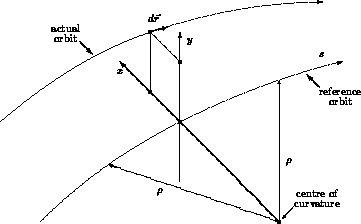
\includegraphics{figures/local_reference.png}
  \caption{\href{local}{Local Reference System}}%{\textbf{Figure 1:} Local Reference System}}
\end{figure}

%%\end{document}
\href{http://www.cern.ch/Hans.Grote/hansg_sign.html}{hansg}, May 8, 2001 

% add other files to the end of this file

%%\title{the mad program}
%  Changed by: Chris ISELIN, 24-Jan-1997 
%  Changed by: Hans Grote, 10-Jun-2002 

\section{Closed Orbit}
\label{sec:closed_orbit}

Due to various errors like misalignment errors, field errors, fringe
fields etc., the closed orbit does not coincide with the reference
orbit. It also changes with the momentum error. The closed orbit is
described with respect to the reference orbit, using the local
reference system (\textit{x, y, s}). It is evaluated including any
nonlinear effects.  

MAD also computes the betatron and synchrotron oscillations with respect
to the closed orbit. Results are given in the local (\textit{x, y,
  s})-system defined by the reference orbit. 


%\href{http://www.cern.ch/Hans.Grote/hansg_sign.html}{hansg}, January 24, 1997 


%%\title{Global Reference System}
%  Changed by: Chris ISELIN, 17-Jul-1997 

%  Changed by: Hans Grote, 10-Jun-2002 

%%\usepackage{hyperref}
% commands generated by html2latex


%%\begin{document}
%%\begin{center}
 %%EUROPEAN ORGANIZATION FOR NUCLEAR RESEARCH 
%%\includegraphics{http://cern.ch/madx/icons/mx7_25.gif}

\subsection{Global Reference System}
%%\end{center} 
 The \hyperlink{global}{global reference orbit} of the accelerator is uniquely defined by the sequence of physical elements. The local reference system (\textit{x}, \textit{y}, \textit{s}) may thus be referred to a global Cartesian coordinate system (\textit{X}, \textit{Y}, \textit{Z}) (see \hyperlink{global}{Figure 1}). The positions between beam elements are numbered 0,...,i,...n. The local reference system  (\textit{x$_i$, y$_i$, s$_i$}) at position \textit{i}, i.e. the displacement and direction of the reference orbit with respect to the system (\textit{X}, \textit{Y}, \textit{Z}) are defined by three displacements  (\textit{X$_i$}, \textit{Y$_i$}, \textit{Z$_i$}) and three angles (\textit{Theta$_i$}, \textit{Phi$_i$}, \textit{Psi$_i$}) The above quantities are defined more precisely as follows: 
\begin{itemize}
	\item X: Displacement of the local origin in \textit{X}-direction. 
	\item Y: Displacement of the local origin in \textit{Y}-direction. 
	\item Z: Displacement of the local origin in \textit{Z}-direction. 
	\item \href{theta}{THETA}: Angle of rotation (azimuth) about the global \textit{Y}-axis, between the global \textit{Z}-axis and the projection of the reference orbit onto the (\textit{Z}, \textit{X})-plane. A positive angle THETA forms a right-hand screw with the \textit{Y}-axis. 
	\item \href{phi}{PHI}: Elevation angle, i.e. the angle between the reference orbit and its projection onto the (\textit{Z}, \textit{X})-plane. A positive angle PHI correspond to increasing \textit{Y}. If only horizontal bends are present, the reference orbit remains in the (\textit{Z}, \textit{X})-plane. In this case PHI is always zero. 
	\item \href{psi}{PSI}: Roll angle about the local \textit{s}-axis, i.e. the angle between the intersection (\textit{x}, \textit{y})- and (\textit{Z}, \textit{X})-planes and the local \textit{x}-axis. A positive angle PSI forms a right-hand screw with the \textit{s}-axis. 
\end{itemize} The angles (THETA, PHI, PSI) are \textbf{not} the Euler angles. The reference orbit starts at the origin and points by default in the direction of the positive \textit{Z}-axis. The initial local axes (\textit{x}, \textit{y}, \textit{s})  coincide with the global axes (\textit{X}, \textit{Y}, \textit{Z}) in this order. The six quantities (X$_0$, Y$_0$, Z$_0$, THETA$_0$, PHI$_0$, PSI$_0$) thus all have zero initial values by default. The program user may however specify different initial conditions. 

 Internally the displacement is described by a vector \textit{V} and the orientation by a unitary matrix \textit{W}. The column vectors of \textit{W} are the unit vectors spanning  the local coordinate axes in the order (\textit{x, y, s}). \textit{V} and \textit{W} have the values: 


%%\includegraphics{null}
%VW
\[
V =
 \begin{pmatrix}
  X \\
  Y \\
  Z
 \end{pmatrix}
, \quad\quad
W=\Theta\Phi\Psi
\]

 where 

%%\includegraphics{null}
%PhiThetaPsi
\[
\Theta =
 \begin{pmatrix}
  \cos \theta & 0 &  \sin \theta \\
  0 & 1 &  0 \\
  -\sin \theta & 0 &  \cos \theta
 \end{pmatrix}
, \quad
\Phi =
 \begin{pmatrix}
  1 & 0 &  0 \\
  0 & \cos \phi &  \sin \phi \\
  0 & -\sin \phi &  \cos \phi
 \end{pmatrix}
, \quad
\Psi =
 \begin{pmatrix}
  \cos \psi &  -\sin \psi & 0 \\
  \sin \psi &  \cos \psi & 0 \\
	0			&	0			 & 1 
 \end{pmatrix}
.
\]

 The reference orbit should be closed and it should not be twisted. This means that the displacement of the local reference system must be periodic with the revolution frequency of the accelerator, while the position angles must be periodic modulo(2 pi) with the revolution frequency. If PSI is not periodic module(2 pi), coupling effects are introduced. When advancing through a beam element, MAD computes \textit{V$_i$} and \textit{W$_i$} by the recurrence relations 

\textit{V$_i$ = W$_i-1$R$_i$ + V$_i-1$}, \textit{W$_i$ = w$_i-1$S$_i$}. 

 The vector \textit{R$_i$} is the displacement and the matrix \textit{S$_i$} is the rotation of the local reference system  at the exit of the element \textit{i} with respect to the entrance  of the same element. The values of \textit{R$_i$} and \textit{S$_i$} are listed in the:   \href{local_system.html#straight}{straight reference system} for each physical element type. 
%%%\begin{center}
%\href{global}{
%%%\includegraphics{null}}
%
%\textbf{Figure 1:} Global Reference System 
%%%\end{center}
\begin{figure}[h!]
  \centering
	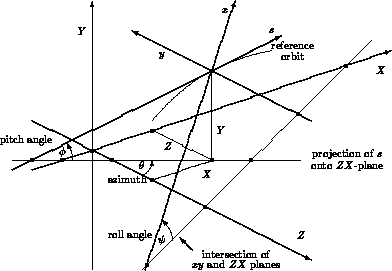
\includegraphics{figures/global.png}
  \caption{\href{global}{Global Reference System }}%{\textbf{Figure 1:} Local Reference System}}
\end{figure}

\href{http://www.cern.ch/Hans.Grote/hansg_sign.html}{hansg}, January 24, 1997 

%%\end{document}

%%\title{Local Reference System}
%  Changed by: Chris ISELIN, 17-Jul-1997 
%  Changed by: Hans Grote, 25-Sep-2002 

\section{Local Reference Systems}

\subsection{\href{straight}{Reference System for Straight Beam
    Elements}} 
In straight elements the local reference system is simply translated by
the length of the element along the local \textit{s}-axis. This is true
for  
\begin{itemize}
   \item \href{drift.html}{Drift space}, 
   \item \href{quadrupole.html}{Quadrupole}, 
   \item \href{sextupole.html}{Sextupole}, 
   \item \href{octupole.html}{Octupole}, 
   \item \href{solenoid.html}{Solenoid}, 
   \item \href{crabcavity.html}{CRABCAVITY}, 
   \item \href{cavity.html}{RF cavity}, 
   \item \href{separator.html}{Electrostatic separator}, 
   \item \href{kickers.html}{Closed orbit corrector}, 
   \item \href{monitors.html}{Beam position monitor}. 
\end{itemize} 

The corresponding \textit{R}, \textit{S} are 
%%\includegraphics{null}
%RSstraight
\[
R =
 \begin{pmatrix}
  0 \\
  0 \\
  L
 \end{pmatrix}
, \quad
S =
 \begin{pmatrix}
  1 & 0 &  0 \\
  0 & 1 &  0 \\
  0 & 0 &  1
 \end{pmatrix}
.
\]

A rotation of the element about the \textit{S}-axis has no effect on
\textit{R} and \textit{S}, since the rotations of the reference system
before and after the element cancel.  
%%\begin{center}
%%\includegraphics{null}
\begin{figure}[H]
  \centering
	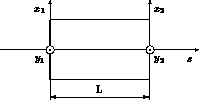
\includegraphics{figures/ref_straight.png}
  \caption{Reference System for Straight Beam Elements}
%\\\textbf{Figure 1:} Reference System for Straight Beam Elements 
\end{figure}


\subsection{\href{rbend}{Reference System for Bending Magnets}}
\href{bend.html}{Bending magnets} have a curved reference orbit. For
both rectangular and sector bending magnets  


%%\includegraphics{null}
%RSbend
\[
R =
 \begin{pmatrix}
  \rho\,(\cos \alpha - 1) \\
  0 \\
  \rho\,\sin \alpha
 \end{pmatrix}
, \quad
S =
 \begin{pmatrix}
  \cos \alpha & 0 &  -\sin \alpha \\
  0 & 1 &  0 \\
  \sin \alpha & 0 &  \cos \alpha
 \end{pmatrix}
,
\]

where alpha is the bend angle. A positive bend angle represents a bend
to the right, i.e. towards negative \textit{x} values. For sector
bending magnets, the bend radius is given by rho, and for rectangular
bending magnets it has the value  

 rho = \textit{L} / 2 sin(alpha/2). 

If the magnet is rotated about the \textit{s}-axis by an angle psi,
\textit{R} and \textit{S} are transformed by  

\textit{R}* = \textit{T R}, \textit{S}* = \textit{T S T$^-1$}. 

where \textit{T} is the orthogonal rotation matrix 


%%\includegraphics{null}
%Trot
\[
T =
 \begin{pmatrix}
  \cos \psi &  -\sin \psi & 0 \\
  \sin \psi &  \cos \psi  & 0 \\
  0	    &	0	  & 1 
 \end{pmatrix}
.
\]

The special value psi = pi/2 represents a bend down.  

%%\begin{center}
%\href{rbend}{
%%%\includegraphics{null}}
\begin{figure}[H]
  \centering
	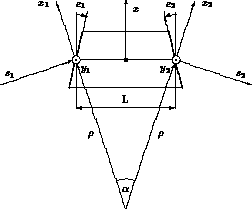
\includegraphics{figures/ref_rbend.png}
  \caption{Reference System for Rectangular Bends; The signs of the pole-face rotations are positive as shown.}
%\\\textbf{Figure 2:} Reference System for Rectangular Bends; The signs of the pole-face rotations are positive as shown. 
\end{figure}

%%\includegraphics{null}}
\begin{figure}[H]
  \centering
	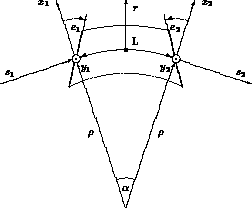
\includegraphics{figures/ref_sbend.png}
  \caption{Reference System for Sector Bends; The signs of the pole-face rotations are positive as shown. }
%\\\textbf{Figure 3:}  Reference System for Sector Bends; The signs of the pole-face rotations are positive as shown. 
\end{figure}


\subsection{Elements which do not Change the Local Reference}
\href{marker.html}{MARKER} elements do not  affect the reference orbit. They are ignored for geometry calculations.  

%\href{http://www.cern.ch/Hans.Grote/hansg_sign.html}{hansg}, January 24, 1997 


% add other files to the end of this file

%%%\title{DRIFT}
%  Changed by: Chris ISELIN, 24-Jan-1997 
%  Changed by: Hans Grote, 30-Sep-2002 

\section{Drift Space}

\begin{verbatim}
label: DRIFT,L=real;
\end{verbatim} 

A DRIFT space has one real attribute: 
\begin{itemize}
   \item L: The drift length (default: 0 m) 
\end{itemize} 

Examples: 
\begin{verbatim}
DR1: DRIFT, L = 1.5;
DR2: DRIFT, L = DR1[L];
\end{verbatim} 

The length of DR2 will always be equal to the length of DR1. The
\href{../Introduction/local_system.html#straight}{straight  reference
  system} for a drift space is a cartesian coordinate system.  

%\href{http://www.cern.ch/Hans.Grote/hansg_sign.html}{hansg}, January 24, 1997 

%%%\title{QUADRUPOLE}
%  Changed by: Chris ISELIN, 27-Jan-1997 
%  Changed by: Hans Grote, 30-Sep-2002 
%  Changed by: Frank Schmidt, 28-Aug-2003 
%  Changed by: Andrea Latina, 6-May-2013 

\section{Quadrupole}

\begin{verbatim}
label: QUADRUPOLE, L = real, K1 = real, K1S = real, TILT = real;
\end{verbatim}    

A QUADRUPOLE has four real attributes:     
\begin{itemize}
   \item L: The quadrupole length (default: 0 m). 
   \item K1: The normal quadrupole coefficient \\        
     \textit{K}$_1$ = 1/(\textit{B} rho) ($\partial$\textit{B$_y$}/$\partial$\textit{x}).\\ 
     The default is 0 m**(-2). A positive normal quadrupole strength
     implies horizontal focussing of positively charged particles.  
   \item K1S: The skew quadrupole coefficient \\        
     \textit{K}$_{1s}$ = 1/(2 \textit{B} rho)
     ($\partial$\textit{B$_x$}/$\partial$\textit{x} -
     $\partial$\textit{B$_y$}/$\partial$\textit{y})\\  
     where (x,y) is now a coordinate system rotated by -45$^o$ around s
     with respect to the normal one. The default is 0  m**(-2). A
     positive skew quadrupole strength implies defocussing (!) of
     positively charged particles in the (x,s) plane rotated by 45$^o$
     around s (particles in this plane have x = y $>$ 0). 
   \item TILT: The roll angle about the longitudinal axis (default: 0
     rad, i.e. a normal quadrupole). A positive angle represents a
     clockwise rotation. A TILT=pi/4 turns a positive normal quadrupole
     into a negative skew quadrupole.          

\textbf{ Please note that contrary to MAD8 one has to
  specify the desired TILT angle, otherwise it is taken as
  0 rad. This was needed to avoid the confusion in MAD8
  about the actual meaning of the TILT attribute for
  various elements. } 

    \item THICK: If this flag is set to 1 the quadrupole will be tracked
      through as a thick-element, instead of being converted into
      thin-lenses.  
\end{itemize}

\textbf{ Note also that K$_1$/K$_{1s}$ can be considered as
  the normal or skew quadrupole components of the magnet on
  the bench, while the TILT attribute can be considered as an
  tilt alignment error in the machine. In fact, a positive
  K$_1$ with a tilt=0 is equivalent to a positive K$_{1s}$
  with positive tilt=+pi/4. } 

Example: 
\begin{verbatim}
QF: QUADRUPOLE, L = 1.5, K1 = 0.001, THICK = 1;
\end{verbatim}     

The \href{local_system.html#straight}{straight reference system} for
a quadrupole is a cartesian coordinate system.

%\href{http://www.cern.ch/Hans.Grote/hansg_sign.html}{hansg},
%\href{http://www.cern.ch/Frank.Schmidt/frs_sign.html}{frs},
%\href{https://phonebook.cern.ch/phonebook/?id=PE525753}{al},       May 6, 2013 

%%%\title{SEXTUPOLE}
%  Changed by: Chris ISELIN, 27-Jan-1997 

%  Changed by: Hans Grote, 30-Sep-2002 

%  Changed by: Frank Schmidt, 28-Aug-2003 

%%\usepackage{hyperref}
% commands generated by html2latex


%%\begin{document}
%%\begin{center}
 %%EUROPEAN ORGANIZATION FOR NUCLEAR RESEARCH 
%%\includegraphics{http://cern.ch/madx/icons/mx7_25.gif}

\subsection{Sextupole}
%%\end{center}
\begin{verbatim}

label: SEXTUPOLE,L=real,K2=real,K2S=real,TILT=real;
\end{verbatim} A SEXTUPOLE has four real attributes: 
\begin{itemize}
	\item L: The sextupole length (default: 0 m). 
	\item K2: The normal sextupole coefficient 

\textit{K}$_2$ = 1/(\textit{B} rho) ($\partial$$^2$\textit{B$_y$}/$\partial$ \textit{x}$^2$). 

 (default: 0 m**(-3)). 
	\item K2S: The skew sextupole coefficient 

\textit{K}$_{2S}$ = 1/(2 \textit{B} rho) ($\partial$$^2$\textit{B$_x$}/$\partial$ \textit{x}$^2$ - $\partial$$^2$\textit{B$_y$}/$\partial$ \textit{y}$^2$). 

 where (x,y) is now a coordinate system rotated by -30$^o$ around s with respect to the normal one. (default: 0 m**(-3)). A positive skew sextupole strength implies defocussing (!) of positively charged particles in the (x,s) plane rotated by 30$^o$ around s (particles in this plane have x $>$ 0, y $>$ 0). 


	\item TILT: The roll angle about the longitudinal axis (default: 0 rad, i.e. a normal sextupole). A positive angle represents a clockwise rotation. A TILT=pi/6 turns a positive normal sextupole into a negative skew sextupole. 

\textbf{  Please note that contrary to MAD8 one has to specify the desired TILT angle, otherwise it is taken as 0 rad. This was needed to avoid the confusion in MAD8 about the actual meaning of the TILT attribute for various elements. }
\end{itemize}

\textbf{  Note also that K$_2$/K$_{2s}$ can be considered as the normal or skew sextupole components of the magnet on the bench, while the TILT attribute can be considered as an tilt alignment error in the machine. In fact, a positive K$_2$ with a tilt=0 is equivalent to a positive K$_{2s}$ with positive tilt=+pi/6.  }

Example: 
\begin{verbatim}

S: SEXTUPOLE,L=0.4,K2=0.00134;
\end{verbatim} The \href{local_system.html#straight}{straight reference system} for a sextupole is a cartesian coordinate system.  

\href{http://www.cern.ch/Hans.Grote/hansg_sign.html}{hansg}, \href{http://www.cern.ch/Frank.Schmidt/frs_sign.html}{frs}, August 28, 2003  

%%\end{document}

%%%\title{the mad program}
%  Changed by: Chris ISELIN, 27-Jan-1997 
%  Changed by: Hans Grote, 30-Sep-2002 
%  Changed by: Frank Schmidt, 28-Aug-2003 

\section{Octupole}

\begin{verbatim}
label: OCTUPOLE, L = real, K3 = real, K3S = real, TILT = real;
\end{verbatim} 

An OCTUPOLE has four real attributes: 
\begin{itemize}
   \item L: The octupole length (default: 0 m). 

   \item K3: The normal octupole coefficient \\
     \textit{K}$_3$ = 1/(\textit{B} rho)
     ($\partial$$^3$\textit{B$_y$}/$\partial$\textit{x}$^3$). \\ 
     (default: 0 m**(-4)). 

   \item K3S: The skew octupole coefficient 
%% 2013-Jul-05  18:00:59  ghislain: to be checked wrt error reported on
%% K2S for sextupoles 
     \textit{K}$_3S$ = 1/(2 \textit{B} rho)
     ($\partial$$^3$\textit{B$_x$}/$\partial$\textit{x}$^3$ -
     $\partial$$^3$\textit{B$_y$}/$\partial$\textit{y}$^3$). \\
     where (x,y) is now a coordinate system rotated by -22.5$^o$ around
     s with respect to the normal one. (default: 0 m**(-4)). A positive
     skew octupole strength implies defocussing (!) of positively
     charged particles in the (x,s) plane rotated by 22.5$^o$ around s
     (particles in this plane have x $>$ 0, y $>$ 0).  

   \item TILT: The roll angle about the longitudinal axis (default: 0
     rad, i.e. a normal octupole). A positive angle represents a
     clockwise rotation. A TILT=pi/8 turns a positive normal octupole
     into a negative skew octupole.  

     \textbf{  Please note that contrary to MAD8 one has to specify the
       desired TILT angle, otherwise it is taken as 0 rad. This was
       needed to avoid the confusion in MAD8 about the actual meaning of
       the TILT attribute for various elements. }

\end{itemize}

\textbf{  Note also that K$_3$/K$_3s$ can be considered as the normal or
  skew quadrupole components of the magnet on the bench, while the TILT
  attribute can be considered as an tilt alignment error in the
  machine. In fact, a positive K$_3$ with a tilt=0 is equivalent to a
  positive K$_3s$ with positive tilt=+pi/8. } 

Example: 
\begin{verbatim}
O3: OCTUPOLE, L = 0.3, K3 = 0.543;
\end{verbatim} 

The \href{local_system.html#straight}{straight reference system} for a
octupole is a cartesian coordinate system. Octupoles are normally
treated as thin lenses, except when tracking by Lie-algebraic methods.   

%\href{http://www.cern.ch/Hans.Grote/hansg_sign.html}{hansg}, 
%\href{http://www.cern.ch/Frank.Schmidt/frs_sign.html}{frs}, August 28, 2003  

%%%\title{SOLENOID}
%  Changed by: Chris ISELIN, 27-Jan-1997 
%  Changed by: Hans Grote, 30-Sep-2002 
%  Changed by: Alexander Koschik, 16-May-2006 

\section{Solenoid}

\texttt{label: SOLENOID, L = real, KS = real;           } (\textbf{thick} version) 
\\
\texttt{label: SOLENOID, L = 0,    KS = real, KSI=real; } (\textbf{thin} version) 

A SOLENOID has two or three real attributes: 
\begin{itemize}
   \item L: The length of the solenoid (default: 0 m) 
   \item KS: The solenoid strength \textit{K$_s$} (default: 0
     rad/m). For positive KS and positive particle charge, the solenoid
     field points in the direction of increasing \textit{s}.  
   \item KSI: The solenoid integrated strength \textit{K$_s$*L}
     (default: 0 rad).  This additional attribute is needed only when
     using the thin solenoid,  where \textit{L=0}!     
   \item \textit{ KNL \& KSL:  Take note that one can specify multipole
     coefficients but they have no effect in MAD-X proper but are used
     for solenoids with multipoles in PTC.} 
\end{itemize}

Example: 
\begin{verbatim}
SOLO: SOLENOID, L = 2., KS = 0.001;
THINSOLO: SOLENOID, L = 0, KS = 0.001, KSI = 0.002;
\end{verbatim}

The \href{local_system.html#straight}{straight reference system} for a
solenoid is a cartesian coordinate system. 
 
%\href{http://www.cern.ch/Hans.Grote/hansg_sign.html}{hansg}, January 27, 1977 

%%%\title{CRABCAVITY}
%  Added by: R. Calaga, Sep 2010 
%  Edited by: A. Latina, Jun 2013

\section{Crab Cavity}


\begin{verbatim}
label: CRABCAVITY, L = real, VOLT = real, LAG = real, FREQ = real,
                   RV1 = integer, RV2 = integer, RV3 = integer, RV4 = integer, 
                   RPH1 = integer, RPH2 = integer, 
                   LAGF = real, HARMON = integer;                 
\end{verbatim} 

%  BETRF=real, PG=real,
%  FREQ=real, SHUNT=real, TFILL=real; 

A CRABCAVITY has five real attributes and seven integer attributes: 

\begin{itemize}
  \item L: The length of the cavity (default: 0 m) 

  \item VOLT: The peak RF voltage (default: 0 MV). 

  \item LAG: The initial phase lag [2pi] (default: 0). 

  \item FREQ: The RF frequency [MHz] (no default). \\
    {\bf Note that if the RF frequency is not given, it is computed from the
    harmonic number and the revolution frequency \textit{f$_0$} as before. 
    However, for deflecting structures this makes no sense, and the 
    frequency is mandatory.} 

  \item RV1: Number of initial turns with zero voltage (default: 0). 
  \item RV2: Number of turns to ramp voltage from zero to nominal value (default: 0). 
  \item RV3: Number of turns with nominal voltage (default: 0). 
  \item RV4: Number of turns to ramp voltage from nominal value to zero (default: 0).  

  \item LAGF: Value of the final crab RF phase lag [2pi] (default: 0).

  \item RPH1: Number of initial turns with nominal phase (default: 0). 
  \item RPH2: Number of turns to ramp phase [2pi] from nominal to
    specified value \\ (default:~0). 

  \item HARMON: The harmonic number \textit{h} (no default). \\
    Only if the frequency is not given. 

% \item BETRF: RF coupling factor (default: 0).
% \item PG: The RF power per cavity (default: 0 MW).
% \item SHUNT: The relative shunt impedance (default: 0 MOhm/m).
% \item TFILL: The filling time of the cavity T<sub>fill</sub> (default: 0 microseconds). 
%\item EPHASE: Value of the final crab RF phase [2pi] with respect to  nominal value (default: 0). 
\end{itemize}


{\bf Caveats:}
\begin{itemize}
   \item \textit{ Please take note, that the following MAD8 attributes:
     BETRF, PG, SHUNT and TFILL are currently not implemented in MAD-X!}
   \item \textit{ Note that crab cavities are only implemented for
     tracking  purposes. \\ TWISS will ignore any effect of the crab cavity.  
% as well that twiss is 4D only. As a consequence the TWISS
% parameters in the plane of non-zero dispersion may not close as
% expected. Therefore, it is best to perform TWISS in 4D only, i.e. with
% cavities switched off. If 6D is needed one has to use the
% 
% <a href="../ptc_twiss/ptc_twiss.html">ptc_twiss</a> command. 
}
\end{itemize} 

%A cavity requires the particle energy (\href{beam.html#energy}{ENERGY})
%and the particle charge (\href{beam.html#charge}{CHARGE}) to be set by
%a \href{beam.html}{BEAM} command before any calculation is performed. 

Before any calculation is performed with a CRABCAVITY, the particle
energy (\href{beam.html#energy}{ENERGY}) and the particle charge
(\href{beam.html#charge}{CHARGE}) must be set by a
\href{beam.html}{BEAM} command.   

Then the effect of the CRABCAVITY on particle coordinates during tracking is
\\
\\ delta(\textit{px})  = VOLT * sin( PHI - OMEGA * t) 
\\ delta(\textit{E})  = -  VOLT * OMEGA * x * cos(PHI - OMEGA * t) 
\\ 
\\ where PHI =  2 $\pi$ * (LAG - HARMON * \textit{f$_0$ t}), 
\\ and OMEGA = 2 $\pi$ * FREQ / \textit{c}
\\
% delta(<i>E</i>) = VOLT * 
% sin(2 pi * (LAG - HARMON * <i>f<sub>0</sub> t</i>)). 


Example: 
\begin{verbatim}
BEAM, PARTICLE = PROTON, ENERGY = 7000.0;
CAVITY:  CRABCAVITY, L = 10.0, VOLT = 5.0, LAG = 0.0, FREQ = 400,
         RV1 = 0, RV2 = 50, RV3 = 1000, RV4 = 50, 
         RPH1 = 100, RPH2 = 500, LAGF = 0.125;
\end{verbatim} 

The \href{local_system.html#straight}{straight reference system} for a
cavity is a cartesian coordinate system.  
 
%\href{http://www.cern.ch/rcalaga}{R. Calaga}, September 2010

%%%\title{RFCAVITY}
%  Changed by: Chris ISELIN, 27-Jan-1997 
%  Changed by: Hans Grote, 30-Sep-2002 

\section{RF Cavity}


\begin{verbatim}
label: RFCAVITY, L = real, VOLT = real, LAG = real, HARMON = integer, FREQ = real;                  
\end{verbatim} 

%  HARMON=integer, BETRF=real,PG=real,
%                  FREQ=real,SHUNT=real,TFILL=real; 


An RFCAVITY has eight real attributes and one integer attribute: 
\begin{itemize}
   \item L: The length of the cavity (DEFAULT: 0 m) 
   \item VOLT: The peak RF voltage (DEFAULT: 0 MV). The effect of the cavity is \\
     delta(\textit{E}) = VOLT * sin(2 pi * (LAG - HARMON * \textit{f$_0$ t})). 
   \item LAG: The phase lag [2pi] (DEFAULT: 0). 
   \item FREQ: The frequency [MHz] (no DEFAULT). Note that if the RF
     frequency is not given, it is computed from the harmonic number and
     the revolution frequency \textit{f$_0$} as before. However, for
     accelerating structures this makes no sense, and the frequency is
     mandatory.  
   \item HARMON: The harmonic number \textit{h} (no DEFAULT). Only if
     the frequency is not given.  
   \item \textit{ Please take note, that the following MAD8 attributes:
     BETRF, PG, SHUNT and TFILL are currently not implemented in MAD-X!}    
%  \item BETRF: RF coupling factor (DEFAULT: 0).
%  \item PG: The RF power per cavity (DEFAULT: 0 MW).
%  \item SHUNT: The relative shunt impedance (DEFAULT: 0 MOhm/m).
%  \item TFILL: The filling time of the cavity $T_{fill}$ (DEFAULT: 0 microseconds). 

   \item \textit{ Note as well that twiss is 4D only. As a consequence
     the TWISS parameters in the plane of non-zero dispersion may not
     close as expected. Therefore, it is best to perform TWISS in 4D
     only, i.e. with cavities switched off. If 6D is needed one has to
     use the \href{../ptc_twiss/ptc_twiss.html}{ptc\_twiss} command. } 
\end{itemize}  

The RFCAVITY has attributes that will only become active in PTC: 
\begin{itemize}
   \item n\_bessel (DEFAULT: 0): \\
     Transverse focussing effects are typically ignored in the cavity in
     MAD-X or even PTC. This effect is being calculated to order n\_bessel,
     with n\_bessel=0 disregarding this effect and with a correct treatment
     when n\_bessel goes to infinty.
   \item no\_cavity\_totalpath (DEFAULT: no\_cavity\_totalpath=false): \\
     flag to choose if in a cavity the transit time factor is considered
     (no\_cavity\_totalpath=false) or if the particle is kept on the
     crest of RF voltage (no\_cavity\_totalpath=true).  
\end{itemize}  

A cavity requires the particle energy (\href{beam.html#energy}{ENERGY})
and the particle charge (\href{beam.html#charge}{CHARGE}) to be set by a
\href{beam.html}{BEAM} command before any calculations are performed.  

 Example: 
\begin{verbatim}
BEAM, PARTICLE = ELECTRON, ENERGY = 50.0;
CAVITY: RFCAVITY, L = 10.0, VOLT = 150.0, LAG = 0.0, HARMON = 31320;
\end{verbatim} 

The \href{local_system.html#straight}{straight reference system} for a
cavity is a cartesian coordinate system.  

%\href{http://www.cern.ch/Hans.Grote/hansg_sign.html}{hansg}, January 24, 1997 

%%%\title{ELSEPARATOR}
%  Changed by: Chris ISELIN, 27-Jan-1997 
%  Changed by: Hans Grote, 30-Sep-2002 
%  Changed by: Frank Schmidt, 28-Aug-2003 

\section{ELSEPARATOR: Electrostatic Separator}

\begin{verbatim}
label: ELSEPARATOR, L = real, EX = real, EY = real, TILT = real;
\end{verbatim} 

An ELSEPARATOR (electrostatic separator) has four real attributes: 
\begin{itemize}
   \item L: The length of the separator (default: 0 m). 
   \item EX: The horizontal electric field strength (default: 0 MV/m). 
     A positive field increases \textit{p$_x$} for positive particles.  
   \item EY: The vertical electric field strength (default: 0 MV/m). 
     A positive field increases \textit{p$_y$} for positive particles.  
   \item TILT: The roll angle about the longitudinal axis (default: 0
     rad). A positive angle represents a clockwise of the electrostatic
     separator.  
\end{itemize} 

A separator requires the particle energy
(\href{beam.html#energy}{ENERGY}) and the particle charge
(\href{beam.html#charge}{CHARGE}) to be set by a \href{beam.html}{BEAM}
command before any calculations are performed.  

Example: 
\begin{verbatim}
BEAM,PARTICLE = POSITRON, ENERGY = 50.0;
SEP: ELSEPARATOR, L = 5.0, EY = 0.5;
\end{verbatim} 

The \href{local_system.html#straight}{straight reference system} for a
separator is a cartesian coordinate system.   

%\href{http://www.cern.ch/Hans.Grote/hansg_sign.html}{hansg}, 
%\href{http://www.cern.ch/Frank.Schmidt/frs_sign.html}{frs}, August 28, 2003  

%%%\title{KICK, HKICK, VKICK}
%  Changed by: Chris ISELIN, 27-Jan-1997 
%  Changed by: Hans Grote, 30-Sep-2002 
%  Changed by: Frank Schmidt, 28-Aug-2003 
%  Changed by: Werner Herr, 22-May-2007 

\section{Closed Orbit Correctors}
  
Three types of closed orbit correctors are available: 
\begin{itemize}
   \item \href{hkick}{HKICKER}, a corrector for the horizontal plane, 
   \item \href{vkick}{VKICKER}, a corrector for the vertical plane, 
   \item \href{kick}{KICKER}, a corrector for both planes. 
\end{itemize}

\begin{verbatim}
label: HKICKER, L = real, KICK = real, TILT = real;
label: VKICKER, L = real, KICK = real, TILT = real;
label:  KICKER, L = real, HKICK = real, VKICK = real, TILT = real;
\end{verbatim} 

{\bf The type KICKER should not be used when an orbit corrector kicks
  only in one plane.}  

The attributes have the following meaning: 
\begin{itemize}
   \item L: The length of the closed orbit corrector (default: 0 m). 
   \item KICK: The kick angle for either horizontal or vertical correctors. (default: 0 rad). 
   \item HKICK: The horizontal kick angle for a corrector in both planes (default: 0 rad). 
   \item VKICK: The vertical kick angle for a corrector in both planes (default: 0 rad). 
   \item TILT: The roll angle about the longitudinal axis (default: 0
     rad). A positive angle represents a clockwise rotation of the
     kicker.  
\end{itemize} 

A positive kick increases \textit{p$_x$} or \textit{p$_y$}
respectively. This means that a positive horizontal kick bends to the
left,  i.e. to positive x which is opposite of what is true for bends.   

It should be noted that the kick values assigned to an orbit corrector
like above are not overwritten by an orbit correction using the CORRECT
command. Instead the kicks computed by an orbit correction and the
assigned values are added when the correctors are used.  

 Examples: 
\begin{verbatim}
HK1:   HKICKER, KICK = 0.001;
VK3:   VKICKER, KICK = 0.0005;
VK4:   VKICKER, KICK := AVK4;
KHV1:  KICKER,  HKICK = 0.001, VKICK = 0.0005;
KHV2:  KICKER,  HKICK := AKHV2H, VKICK := AKHV2V;
\end{verbatim} 

The assignment in the form of a deferred expression has the advantage
that the values can be assigned and/or modified at any time (and matched
!).  

The \href{local_system.html#straight}{straight reference system} for an
orbit corrector is a Cartesian coordinate s ystem.  

Please note that there is a new feature introduced by Stefan Sorge from
GSI. Here his decription:

The elements KICKER, HKICKER, and VKICKER can also be used as  an
exciter providing a sinusoidal momentum kick. The usage in this case is   

\begin{verbatim}
xykick: KICKER,  SINKICK = integer, SINPEAK = real, SINTUNE = real, SINPHASE = real;  
xkick : HKICKER, SINKICK = integer, SINPEAK = real, SINTUNE = real, SINPHASE = real;  
ykick : VKICKER, SINKICK = integer, SINPEAK = real, SINTUNE = real, SINPHASE = real;  
\end{verbatim}
where a sinusoidal momentum kick dpz as a function of the  revolution
number n given by\\   
dpz(n)=SINPEAK * sin(2*PI*SINTUNE*n + SINPHASE), pz=px,py \\ 
is provided. 

The variables are 

\begin{itemize}
   \item SINKICK - integer, must be set to 1 to switch on the sinusoidal
     signal, default: 0.  
   \item SINPEAK - amplitude of the bending angle (rad), default: 0 rad.  
   \item SINTUNE - frequency of the signal times the revolution
     frequency.  Hence, the phase per revolution is 2*PI*SINTUNE,
     default: 0.   
   \item SINPHASE - initial phase, default: 0 rad.  
   \item KICKER generates a kick in horizontal and a kick vertical
     direction,  where both are synchron, HKICKER generates a horizontal
     kick,  and VKICKER generates a vertical kick.   
\end{itemize}

The momentum kick of a kicker has only a single frequency. An element
having a finite bandwidth can approximately created by defining  thin
kickers with all amplitudes SINPEAK, frequencies SINTUNE, and  initial
phases SINPHASE desired and putting them at the same position s in  the
accelerator.   

From S.Sorge@gsi.de  

%\href{http://www.cern.ch/Hans.Grote/hansg_sign.html}{hansg}, 
%\href{http://www.cern.ch/Frank.Schmidt/frs_sign.html}{frs}, August 28, 2003  

%%%\title{Monitors}
%  Changed by: Chris ISELIN, 27-Jan-1997 
%  Changed by: Hans Grote, 30-Sep-2002 
%  Changed by: G. Roy, 17 Oct 2013: added PLACEHOLDER

\section{Beam Position Monitors}
\label{sec:monitors}

A beam monitor acts on the beam like a drift space. In addition it
serves to record the beam position for closed orbit corrections. Four
different types of beam position monitors are recognised:  

\begin{itemize}
   \item \href{hmon}{HMONITOR}. Monitor for the horizontal beam position, 
   \item \href{vmon}{VMONITOR}. Monitor for the vertical beam position, 
   \item \href{mon}{MONITOR}. Monitor for both horizontal and vertical beam position. 
   \item \href{inst}{INSTRUMENT}. A place holder for any type of beam
     instrumentation. Optically it behaves like a drift space; it
     returns \emph{no beam observation}. It represent a class of
     elements which is completely independent from drifts and monitors.  
   \item \href{plac}{PLACEHOLDER}. A place holder for any type of
     element. Internally it is equivalent to an INSTRUMENT: optically it
     behaves as a drift space, it returns \emph{no beam observation}. It
     represent a class of elements which is completely independent from
     drifts and monitors. 
\end{itemize}

\begin{verbatim}
label: HMONITOR,    L = real;
label: VMONITOR,    L = real;
label: MONITOR,     L = real;
label: INSTRUMENT,  L = real;
label: PLACEHOLDER,  L = real;
\end{verbatim} 

A beam position monitor has one real attribute: 
\begin{itemize}
   \item L: The length of the monitor (default: 0 m). If the length is
     different from zero, the beam position is recorded in the centre of
     the monitor.  
\end{itemize} 

Examples: 
\begin{verbatim}
MH: HMONITOR, L = 1;
MV: VMONITOR;
\end{verbatim} 

The \href{local_system.html#straight}{straight reference system} for a
monitor is a cartesian coordinate system.  

%\href{http://www.cern.ch/Hans.Grote/hansg_sign.html}{hansg}, June 17, 2002 


%%\title{Sign Conventions}
%  Changed by: Chris ISELIN, 17-Jul-1997 
%  Changed by: Hans Grote, 10-Jun-2002 

\section{Sign Conventions for Magnetic Fields}
\label{sec:sign_convention}

The MAD program uses the following Taylor expansion for the field on the
mid-plane \textit{y}=0, described in
\href{bibliography.html#slac75}{SLAC-75}:  


%%\includegraphics{null}
%Taylor_field
$$
B_y(x,0)=\sum_{n=0}^{\infty} \frac{B_n\,x^n}{n!}
$$

Note the factorial in the denominator. The field coefficients have the following meaning: 
\begin{itemize}
   \item \textit{B}$_0$: Dipole field, with a positive value in the
     positive \textit{y} direction; a positive field bends a positively
     charged particle to the right.  
   \item \textit{B}$_1$: Quadrupole coefficient \\
%     \textit{B}$_1$ = (del \textit{B$_y$} / del \textit{x});\\ 
     \( \textit{B}_1 = ( \partial \textit{B}_y / \partial \textit{x} ) \);\\ 
     a positive value corresponds to horizontal focussing of a
     positively charged particle. 
   \item \textit{B}$_2$: Sextupole coefficient \\
%     \textit{B}$_2$ =  (del$^2$\textit{B$_y$} / del \textit{x}$^2$). 
     \( \textit{B}_2 =  ( \partial^2 \textit{B}_y / \partial \textit{x}^2 ) \). 
   \item \textit{B}$_3$: Octupole coefficient \\ 
%     \textit{B}$_3$ =  (del$^3$\textit{B$_y$} / del \textit{x}$^3$). 
     \( \textit{B}_3 =  ( \partial^3 \textit{B}_y / \partial \textit{x}^3 ) \). 
   \item \ldots
\end{itemize} 

Using this expansion and the curvature \textit{h} of the reference
orbit, the longitudinal component of the vector potential to order 4 is:  
%%\includegraphics{null}
%Taylor_A_s
% this is problematic, {align}, {eqnarray} do not work 
% EDIT : Laurent fixed that.
\[
\begin{aligned}
A_x =
&+ B_0\,\Big(x-\frac{hx^2}{2(1+hx)}\Big)&
&+ B_1\,\Big(\frac{1}{2}(x^2-y^2) - \frac{h}{6}x^3 + \frac{h^2}{24}(4x^4-y^4)+\cdots\Big) \\
&+ B_2\,\Big(\frac{1}{6}(x^3-3xy^2) - \frac{h}{24}(x^4-y^4)+\cdots \Big)&
&+ B_3\,\Big(\frac{1}{24}(x^4-6x^2y^2+y^4) \cdots \Big)+\cdots
\end{aligned}
\]

Taking \(\vec{B} = \nabla \times \vec{A}\) in curvilinear coordinates,
the field components can be computed as  

%%\includegraphics{null}
%Taylor_B
\[
\begin{aligned}
B_x(x,y) =
&+ B_1\,\Big(y+\frac{h^2}{6}y^3+\cdots\Big)&  &  \\
&+ B_2\,\Big(xy - \frac{h^3}{6}y^3+\cdots \Big)&+B_3\,\Big(\frac{1}{6}(3x^2y-y^3)+ \cdots \Big)+\cdots\\
B_y(x,y)=
&+ B_0 & + B_1\,\Big(x-\frac{h}{2}y^2+\frac{h^2}{2}xy^2+\cdots \Big)\\
&+ B_2\,\Big(\frac{1}{2}(x^2-y^2)-\frac{h}{2}xy^2+\cdots \Big) & + B_3\,\Big(\frac{1}{6}(x^3-3xy^2)+ \cdots \Big)+\cdots
\end{aligned}
\]

It can be easily verified that both \(\nabla \times \vec{\textit{B}}\)
and \(\nabla . \vec{\textit{B}}\) are zero to the order of the
\(\textit{B}_3\) term.  

Introducing the magnetic rigidity \(\textit{B}\rho = p_s / q\) as the
momentum of the particle divided by its charge, the multipole
coefficients are computed as   
%\textit{K$_n$} = \textit{e B$_n$ / p$_s$} =  \textit{B$_n$ / B} rho. 
\[ \textit{K}_n = \textit{q B}_n / \textit{p}_s  =  \textit{B}_n / \textit{B} \rho \] 


%\href{http://www.cern.ch/Hans.Grote/hansg_sign.html}{hansg}, June 17, 2002 


\chapter{Table Handling Statements} 
\label{chap:tables}

\section{CREATE}
\label{sec:create}
\madbox{
CREATE, TABLE=tabname, COLUMN= var\{, var\} \{, \_name\} ;
}
creates a table with the specified variables as columns. 
The table created is initially empty and can be subsequently
\hyperref[sec:fill]{filled}, and eventually
\hyperref[sec:write]{written} to file in
\hyperref[chap:tfs]{\texttt{TFS}} format.

The special variable name attribute \texttt{\_name} (name preceded by
underscore) adds the element name to the table at the specified column. 


\section{DELETE}
\label{sec:delete}
\madbox{
DELETE, SEQUENCE=seqname, TABLE=tabname;
}
deletes a sequence with name \texttt{seqname} or a table with name
\texttt{tabname} from memory. The sequence deletion is done without
influence on other sequences that may have elements that werein common
with the deleted sequence.

\section{READTABLE}
\label{sec:readtable}
\madbox{
READTABLE, FILE="filename";
}
reads the \texttt{TFS} file \texttt{filename} containing a \mad table
and loads the table into memory with the name specified in the
information section of the TFS file. The table can then be manipulated
as any other table, \textsl{i.e.} its values can be accessed, its data
can be plotted or changed, and it can be written out again. 

\section{READMYTABLE}
\label{sec:readmytable}
\madbox{
READMYTABLE, FILE="filename", TABLE=tabname;
}
reads a \texttt{TFS} file \texttt{filename} containing a \mad table and
loads the table into memory with the name \texttt{tabname}. The table
can then be manipulated as any other table, \textsl{i.e.} its values can
be accessed, its data can be plotted or changed, and it can be written
out again. 

An internal name for the table can be freely assigned, while for the
command \hyperref[sec:readtable]{\texttt{READTABLE}} the table name is
taken from the information section of the table itself.  
This feature allows to store multiple tables of the same type in memory
without overwriting existing ones.   

\section{WRITE}
\label{sec:write}
\madbox{
WRITE, TABLE=tabname, FILE="filename";
}
writes the table "tabname" onto the file "filename"; only the rows and
columns of a preceding \texttt{SELECT, FLAG=table,...;} are written. 
If no \texttt{SELECT} has been issued for this table, only the header is
written to file.
If the FILE argument is omitted, the table is written to standard output.  


%\href{http://www.cern.ch/Hans.Grote/hansg_sign.html}{hansg}, June 17, 2002 

\section{SETVARS}
\label{sec:setvars}

The \texttt{SETVARS} command sets the variables with values extracted
from the row of a table.

\madbox{
SETVARS, TABLE=tabname, ROW=integer;
}

The attributes of \texttt{SETVARS} are:
\begin{madlist}
  \ttitem{TABLE} the name of the table. (Default: none)
  \ttitem{ROW} the row number containing the values. (Default: -1)
\end{madlist}

Negative \texttt{ROW} values are allowed and count the row numbers from
the last row, allowing access to the table in reverse order of rows:
\texttt{ROW~=~-1} accesses the last row of the table,
\texttt{ROW~=~-2} accesses the penultimate (one before last) row,
etc\ldots  

Trying to access the table forward beyond the last row, i.e. \texttt{ROW}
strictly greater than \texttt{nrow} the number of rows in the table, or
trying to access the table backwards before the first row, i.e. \texttt{ROW}
strictly lower than \texttt{-nrow}, or trying to access the illegal
\texttt{ROW=0}, all result in a ``row out of bound'' message and no
variable values are returned and set.  

%% If \texttt{nrow} is the number of rows in the table, the conditions
%% \texttt{ROW $>$ nrow}, ie trying to access the table forward beyond the
%% last row, or \texttt{ROW $<$ -nrow}, ie trying to access the table
%% backwards before the first row, or \texttt{ROW=0} 
%% result in a ``row out of bound'' message and no variable values are
%% returned and set. 


\section{SETVARS\_LIN}
\label{sec:setvars-lin}

The \texttt{SETVARS\_LIN} command sets the variables with values calculated
by linear interpolation, or extrapolation, between two rows of a table. 

\madbox{
  SETVARS\_LIN, \=TABLE=tabname, \\
                \>ROW1=integer, ROW2=integer, PARAM=string;
}

The attributes of \texttt{SETVARS\_LIN} are:
\begin{madlist}
  \ttitem{TABLE} the name of the table. (Default: none)
  \ttitem{ROW1} a first row number with values for interpolation. (Default: 0)
  \ttitem{ROW2} a second row number with values for interpolation. (Default: 0)
  \ttitem{PARAM} a string containing the linear interpolation factor or
  the name of a variable or expression containing the interpolation
  factor. If the resulting value of \texttt{PARAM} is outside the
  $[0,1]$ interval, the result is a linear extrapolation. \\
  (Default: "interp", itself defaulting to a value of 0.0 when evaluated)
\end{madlist}

\texttt{SETVARS\_LIN} sets the variables with values calculated through
the following formula that \madx constructs internally as a deferred
expression which is immediately evaluated:
\madxmp{value := value(row1)*(1-param) + value(row2)*param;}
Both the expression and the value of the expression are available to the
user through respectively the commands \hyperref[sec:show]{\texttt{SHOW}} 
and \hyperref[sec:value]{\texttt{VALUE}}.

When the values are represented as strings, \textsl{e.g.} the name or 
keyword of elements, the resulting value is the string in \texttt{ROW1}.

Negative \texttt{ROW\textit{i}} values are allowed and count the row
numbers from the last row, allowing access to the table in reverse order
of rows: 
\texttt{ROW\textit{i}~=~-1} accesses the last row of the table,
\texttt{ROW\textit{i}~=~-2} accesses the penultimate (one before last)
row, etc\ldots  

Trying to access the table forward beyond the last row,
i.e. \texttt{ROW\textit{i}} strictly greater than \texttt{nrow} the
number of rows in the table, or trying to access the table backwards
before the first row, i.e. \texttt{ROW\textit{i}} strictly lower than
\texttt{-nrow}, or trying to access the illegal
\texttt{ROW\textit{i}=0}, all result in a ``row out of bound'' message
and the expression is not constructed or evaluated. 

\textbf{Example:}
\madxmp{
!  extracts the position of the centre of each element from a standard \\
!  TWISS table giving positions at end of elements: \\
len = table(twiss,tablelength); \\
interpolate = 0.5; \\
i = 2;\\
WHILE \=(i < len) \{ \\
      \>SETVARS\_LIN, TABLE=twiss, ROW1=i-1, ROW2=i, PARAM=interpolate; \\
      \>! now variables are interpolated at the center of the elements. \\
      \>! in particular S holds the position of the center of the element. \\
      \>SHOW, s; VALUE, s; \\
      \>\ldots \\ 
      \>i = i + 1; \};
}

\section{FILL} 
\label{sec:fill}
The \texttt{FILL} command fills a row of a table with the current values 
of all declared column variables of the table.
\madbox{
FILL, TABLE=tabname, ROW=integer;
}

The \texttt{FILL} command takes two arguments:
\begin{madlist}
  \ttitem{TABLE} is the name of the table to be filled. The table must
  have been \hyperref[sec:create]{created} beforehand. 
  The table can then be \hyperref[sec:write]{written} to file in
  \texttt{TFS} format. 

  \ttitem{ROW} is the row number to be filled with the current values of 
  all column variables. \\ 
  \texttt{ROW=0}, or \texttt{ROW=nrow + 1}, where \texttt{nrow} is the
  current number of rows in the table, causes \texttt{FILL} to add a row at
  the end of the table and fill it with the current values of all
  column variables. \\ (Default: 0) 
\end{madlist}

Negative \texttt{ROW} values are allowed and count the row numbers from
the last row, allowing access to the table in reverse order of rows:
\texttt{ROW = -1} accesses the last row of the table,
\texttt{ROW = -2} accesses the penultimate (one before last) row,
etc\ldots  

Trying to access the table forward beyond the last row, i.e. \texttt{ROW}
strictly greater than \texttt{nrow + 1}, where \texttt{nrow} is the number of
rows in the table, or trying to access the table backwards before the
first row, i.e. \texttt{ROW} strictly lower than \texttt{-nrow}, both
result in a ``row out of bound'' message and no values are filled in the
table. 

%% If \texttt{nrow} is the number of rows in the table, the conditions
%% \texttt{ROW $>$ nrow}, ie trying to access the table forward beyond the
%% last row, or \texttt{ROW $<$ -nrow}, ie trying to access the table
%% backwards before the first row, result in a ``row out of bound'' message
%% and no values are filled in the table.

\textbf{Reminder:} One can get access to the current number of rows in a
table using the variable \madxmp{TABLE(tablenanme, TABLELENGTH)}

%% See as well the \href{../Introduction/select.html#ucreate}{user
%% table} example.   

\section{SHRINK} 
\label{sec:shrink}
The \texttt{SHRINK} command removes a number of rows at the end of a table.
\madbox{
SHRINK, TABLE=tabname, ROW=integer;
}

The \texttt{SHRINK} command takes two arguments:
\begin{madlist}
  \ttitem{TABLE} is the name of the table from which rows should be removed. 
  The table must have been previously \hyperref[sec:create]{created} and 
  \hyperref[sec:fill]{filled} or read from file with
  \hyperref[sec:readtable]{\texttt{READTABLE}}
  or \hyperref[sec:readmytable]{\texttt{READMYTABLE}}.
	   
  \ttitem{ROW} is the number of the last row to be kept in the table. 
  All rows beyond the given row number are removed. \\
  Negative values are allowed and count the row numbers from
  the last row, allowing access to the table in reverse order of rows:
  \texttt{ROW~=~-1} removes the last row of the table,
  \texttt{ROW~=~-2} removes the last two rows of the table,
  etc\ldots  \\ 
  (Default: -1) 
\end{madlist}

Trying to access the table forward beyond the last row, i.e. \texttt{ROW}
strictly greater than \texttt{nrow}, where \texttt{nrow} is the number of
rows in the table, or trying to access the table backwards before the
first row, \textsl{i.e.} \texttt{ROW} strictly lower than \texttt{-nrow},
both result in a ``row out of bound'' message and no values are filled
in the table. 


%% \section{SELECT} 
%% \label{sec:select}

%% \begin{verbatim}
%% select, flag=string, range=string, class=string, pattern=string,
%%         sequence=string, full, clear,
%%         column = string{, string},  slice=integer, thick=logical;
%% \end{verbatim} 
%% selects one or several elements for special treatment in a subsequent
%% command based on selection criteria.

%% The selection criteria on a single SELECT statement are logically
%% ANDed, in other words, selected elements have to fulfill the \texttt{RANGE},
%% \texttt{CLASS}, and \texttt{PATTERN} criteria.  
%% The selection criteria on different SELECT statements are logically
%% ORed, in other words selected elements have to fulfill any of the
%% selection criteria accumulated by the different statements.   
%% All selections for a given command remain valid until the "clear" argument
%% is specified; 

%% The "flag" argument allows a determination of the applicability of the
%% SELECT statement and can be one of the following: 
%% \begin{madlist}
%%    \ttitem{seqedit} selection of elements for the
%%      \href{seqedit.html}{seqedit} module.  
%%    \ttitem{error} selection of elements for the
%%      \href{../error/error.html}{error} assignment module.  
%%    \ttitem{makethin} selection of elements for the
%%      \href{../makethin/makethin.html}{makethin} module that
%%      converts the sequence into one with thin elements only.  
%%    \ttitem{sectormap} selection of elements for the
%%      \href{../Introduction/sectormap.html}{sectormap} output file
%%      from the Twiss module.  
%%    \ttitem{save} selection of elements for the \texttt{SAVE} command.  
%%    \ttitem{table} is a table name such as \texttt{twiss}, \texttt{track}
%%      etc., and the rows and columns to be written are selected.  
%% \end{madlist} 

%% The statement
%% \begin{verbatim}
%% SELECT, FLAG=name, FULL;
%% \end{verbatim} 
%% selects ALL positions in the sequence for the flag "name". This is the default
%% for flags for all tables and \texttt{MAKETHIN}.

%% The statement 
%% \begin{verbatim}
%% SELECT, FLAG=name, CLEAR;
%% \end{verbatim} 
%% deselects ALL positions in the sequence for the flag "name". This is the default
%% for flags \texttt{ERROR} and \texttt{SEQEDIT}.

%% "slice" is only used by \href{../makethin/makethin.html}{makethin} and
%% prescribes the number of slices into which the selected elements have to
%% be cut (default = 1).  

%% "column" is only valid for tables and determines the selection of columns
%% to be written into the TFS file. The "name" argument is special in that
%% it refers to the actual name of the selected element. For an example,
%% see \href{../Introduction/select.html}{SELECT}.  

%% "thick" is used to determine whether the selected elements will be
%% treated as thick elements by the MAKETHIN command. This only applies to
%% QUADRUPOLES and BENDS for which thick maps have been explicitely
%% derived. (see ...) 
%% %%2014-Apr-08  17:43:44  ghislain:  A completer.

%% Example: 
%% \begin{verbatim}
%% select, flag = error, class = quadrupole, range = mb[1]/mb[5];
%% select, flag = error, pattern = "^mqw.*";
%% \end{verbatim} 
%% selects all quadrupoles in the range mb[1] to mb[5], as well as all
%% elements (in the whole sequence) with name starting with "mqw", for 
%% treatment by the error module.  

%% Example:  
%% \begin{verbatim}
%% select, flag=save, class=variable, pattern="abc.*";
%% save, file=mysave;
%% \end{verbatim} 
%% will save all variables (and sequences) containing "abc" in their name.
%% However note that since the element class "variable" does not exist, any
%% element with name containing "abc" will not be saved. 

%% \vskip 1cm
%% \hrule
%% \vskip 1cm

%% %% Imported from chapter 2
%% %\subsection{Selection Statements}

%% The elements, or a range of elements, in a sequence can be selected for
%% various purposes. Such selections remain valid until cleared (in
%% difference to \madeight); it is therefore recommended to always start with a  

%% \begin{verbatim}
%% select, flag =..., clear;
%% \end{verbatim} 
%% before setting a new selection. 
%% \begin{verbatim}
%% SELECT, FLAG=name, RANGE=range, CLASS=class, PATTERN=pattern [,FULL] [,CLEAR];
%% \end{verbatim} 
%% where the name for FLAG can be one of ERROR, MAKETHIN, SEQEDIT or the
%% name of a twiss table which is established for all sequence positions in
%% general.  

%% Selected elements have to fulfill the \href{ranges.html#range}{RANGE},
%% \href{ranges.html#class}{CLASS}, and \href{wildcard.html}{PATTERN}
%% criteria.  

%% Any number of SELECT commands can be issued for the same flag and are
%% accumulated (logically ORed). In this context note the following:  

%% \begin{verbatim}
%% SELECT, FLAG=name, FULL;
%% \end{verbatim} 
%% selects all positions in the sequence for this flag. This is the default
%% for all tables and makethin, whereas for ERROR and SEQEDIT the default
%% is "nothing selected".  

%% %\href{save_select}{}
%% \label{save_select}
%% SAVE: A SELECT,FLAG=SAVE statement causes the
%% selected sequences, elements, and variables to be written into the save
%% file. A class (only used for element selection), and a pattern can be
%% specified. Example:  
%% \begin{verbatim}
%% select, flag=save, class=variable, pattern="abc.*";
%% save, file=mysave;
%% \end{verbatim} 
%% will save all variables (and sequences) containing "abc" in their name,
%% but not elements with names containing "abc" since the class "variable"
%% does not exist (astucieux, non ?).  

%% SECTORMAP: A SELECT,FLAG=SECTORMAP statement causes sectormaps to be
%% written into the file "sectormap" like in \madeight. For the file to be
%% written, a flag SECTORMAP must be issued on the TWISS command in
%% addition.  

%% TWISS: A SELECT,FLAG=TWISS statement causes the selected rows and
%% columns to be written into the Twiss TFS file (former OPTICS command in
%% \madeight). The column selection is done on the same select. See as well
%% example 2.  

%% %% Example 1:  
%% %% \begin{verbatim}
%% %% TITLE,'Test input for MAD-X';

%% %% option,rbarc=false; // use arc length of rbends
%% %% beam; ! sets the default beam for the following sequence
%% %% option,-echo;
%% %% call file=fv9.opt;  ! contains optics parameters
%% %% call file="fv9.seq"; ! contains a small sequence "fivecell"
%% %% OPTION,ECHO;
%% %% SELECT,FLAG=SECTORMAP,clear;
%% %% SELECT,FLAG=SECTORMAP,PATTERN="^m.*";
%% %% SELECT,FLAG=TWISS,clear;
%% %% SELECT,FLAG=TWISS,PATTERN="^m.*",column=name,s,betx,bety;
%% %% USE,PERIOD=FIVECELL;
%% %% twiss,file=optics,sectormap;
%% %% stop;
%% %% \end{verbatim} 

%% %% This produces a file \href{sectormap.html}{sectormap}, and a
%% %% twiss output file \label{tfs} (name = optics):  
%% %% \begin{verbatim}
%% %% @ TYPE             %05s "TWISS"
%% %% @ PARTICLE         %08s "POSITRON"
%% %% @ MASS             %le          0.000510998902
%% %% @ CHARGE           %le                       1
%% %% @ E0               %le                       1
%% %% @ PC               %le           0.99999986944
%% %% @ GAMMA            %le           1956.95136738
%% %% @ KBUNCH           %le                       1
%% %% @ NPART            %le                       0
%% %% @ EX               %le                       1
%% %% @ EY               %le                       1
%% %% @ ET               %le                       0
%% %% @ LENGTH           %le                   534.6
%% %% @ ALFA             %le        0.00044339992938
%% %% @ ORBIT5           %le                      -0
%% %% @ GAMMATR          %le           47.4900022541
%% %% @ Q1               %le           1.25413071556
%% %% @ Q2               %le           1.25485338377
%% %% @ DQ1              %le           1.05329608302
%% %% @ DQ2              %le           1.04837000224
%% %% @ DXMAX            %le           2.17763211131
%% %% @ DYMAX            %le                       0
%% %% @ XCOMAX           %le                       0
%% %% @ YCOMAX           %le                       0
%% %% @ BETXMAX          %le            177.70993499
%% %% @ BETYMAX          %le           177.671582415
%% %% @ XCORMS           %le                       0
%% %% @ YCORMS           %le                       0
%% %% @ DXRMS            %le           1.66004270906
%% %% @ DYRMS            %le                       0
%% %% @ DELTAP           %le                       0
%% %% @ TITLE            %20s "Test input for MAD-X"
%% %% @ ORIGIN           %16s "MAD-X 0.20 Linux"
%% %% @ DATE             %08s "07/06/02"
%% %% @ TIME             %08s "14.25.51"
%% %% * NAME               S                  BETX               BETY               
%% %% $ %s                 %le                %le                %le                
%% %%  "MSCBH"             4.365              171.6688159        33.31817319       
%% %%  "MB"                19.72              108.1309095        58.58680717       
%% %%  "MB"                35.38              61.96499987        102.9962313       
%% %%  "MB"                51.04              34.61640793        166.2227523       
%% %%  "MSCBV.1"           57.825             33.34442808        171.6309057       
%% %%  "MB"                73.18              58.61984637        108.0956006       
%% %%  "MB"                88.84              103.0313887        61.93159422       
%% %%  "MB"                104.5              166.2602486        34.58939635       
%% %%  "MSCBH"             111.285            171.6688159        33.31817319       
%% %%  "MB"                126.64             108.1309095        58.58680717       
%% %%  "MB"                142.3              61.96499987        102.9962313       
%% %%  "MB"                157.96             34.61640793        166.2227523       
%% %%  "MSCBV"             164.745            33.34442808        171.6309057       
%% %%  "MB"                180.1              58.61984637        108.0956006       
%% %%  "MB"                195.76             103.0313887        61.93159422       
%% %%  "MB"                211.42             166.2602486        34.58939635       
%% %%  "MSCBH"             218.205            171.6688159        33.31817319       
%% %%  "MB"                233.56             108.1309095        58.58680717       
%% %%  "MB"                249.22             61.96499987        102.9962313       
%% %%  "MB"                264.88             34.61640793        166.2227523       
%% %%  "MSCBV"             271.665            33.34442808        171.6309057       
%% %%  "MB"                287.02             58.61984637        108.0956006       
%% %%  "MB"                302.68             103.0313887        61.93159422       
%% %%  "MB"                318.34             166.2602486        34.58939635       
%% %%  "MSCBH"             325.125            171.6688159        33.31817319       
%% %%  "MB"                340.48             108.1309095        58.58680717       
%% %%  "MB"                356.14             61.96499987        102.9962313       
%% %%  "MB"                371.8              34.61640793        166.2227523       
%% %%  "MSCBV"             378.585            33.34442808        171.6309057       
%% %%  "MB"                393.94             58.61984637        108.0956006       
%% %%  "MB"                409.6              103.0313887        61.93159422       
%% %%  "MB"                425.26             166.2602486        34.58939635       
%% %%  "MSCBH"             432.045            171.6688159        33.31817319       
%% %%  "MB"                447.4              108.1309095        58.58680717       
%% %%  "MB"                463.06             61.96499987        102.9962313       
%% %%  "MB"                478.72             34.61640793        166.2227523       
%% %%  "MSCBV"             485.505            33.34442808        171.6309057       
%% %%  "MB"                500.86             58.61984637        108.0956006       
%% %%  "MB"                516.52             103.0313887        61.93159422       
%% %%  "MB"                532.18             166.2602486        34.58939635       
%% %% \end{verbatim}

%%  %% Example 2: 

%% %%  Addition of variables to (any internal) table: 
%% %% \begin{verbatim}
%% %% select, flag=table, column=name, s, betx, ..., var1, var2, ...; ! or
%% %% select, flag=table, full, column=var1, var2, ...; ! default col.s + new
%% %% \end{verbatim} 
%% %% will write the current value of var1 etc. into the table each time a new
%% %% line is added; values from the same (current) line can be accessed by
%% %% these variables, e.g.  
%% %% \begin{verbatim}
%% %% var1 := sqrt(beam->ex*table(twiss,betx));
%% %% \end{verbatim} 
%% %% in the case of table above being "twiss". The plot command accepts the
%% %% new variables.  

%% %% Remark: this replaces the "string" variables of MAD-8. 

%% %%  This example demonstrates as well the usage of a user defined table \label{ucreate}. 
%% %% \begin{verbatim}
%% %% beam,ex=1.e-6,ey=1.e-3;
%% %% // element definitions
%% %% mb:rbend, l=14.2, angle:=0,k0:=bang/14.2;
%% %% mq:quadrupole, l:=3.1,apertype=ellipse,aperture={1,2};
%% %% qft:mq, l:=0.31, k1:=kqf,tilt=-pi/4;
%% %% qf.1:mq, l:=3.1, k1:=kqf;
%% %% qf.2:mq, l:=3.1, k1:=kqf;
%% %% qf.3:mq, l:=3.1, k1:=kqf;
%% %% qf.4:mq, l:=3.1, k1:=kqf;
%% %% qf.5:mq, l:=3.1, k1:=kqf;
%% %% qd.1:mq, l:=3.1, k1:=kqd;
%% %% qd.2:mq, l:=3.1, k1:=kqd;
%% %% qd.3:mq, l:=3.1, k1:=kqd;
%% %% qd.4:mq, l:=3.1, k1:=kqd;
%% %% qd.5:mq, l:=3.1, k1:=kqd;
%% %% bph:hmonitor, l:=l.bpm;
%% %% bpv:vmonitor, l:=l.bpm;
%% %% cbh:hkicker;
%% %% cbv:vkicker;
%% %% cbh.1:cbh, kick:=acbh1;
%% %% cbh.2:cbh, kick:=acbh2;
%% %% cbh.3:cbh, kick:=acbh3;
%% %% cbh.4:cbh, kick:=acbh4;
%% %% cbh.5:cbh, kick:=acbh5;
%% %% cbv.1:cbv, kick:=acbv1;
%% %% cbv.2:cbv, kick:=acbv2;
%% %% cbv.3:cbv, kick:=acbv3;
%% %% cbv.4:cbv, kick:=acbv4;
%% %% cbv.5:cbv, kick:=acbv5;
%% %% !mscbh:sextupole, l:=1.1, k2:=ksf;
%% %% mscbh:multipole, knl:={0,0,0,ksf},tilt=-pi/8;
%% %% mscbv:sextupole, l:=1.1, k2:=ksd;
%% %% !mscbv:octupole, l:=1.1, k3:=ksd,tilt=-pi/8;

%% %% // sequence declaration

%% %% fivecell:sequence, refer=centre, l=534.6;
%% %%    qf.1:qf.1, at=1.550000e+00;
%% %%    qft:qft, at=3.815000e+00;
%% %% !   mscbh:mscbh, at=3.815000e+00;
%% %%    cbh.1:cbh.1, at=4.365000e+00;
%% %%    mb:mb, at=1.262000e+01;
%% %%    mb:mb, at=2.828000e+01;
%% %%    mb:mb, at=4.394000e+01;
%% %%    bpv:bpv, at=5.246000e+01;
%% %%    qd.1:qd.1, at=5.501000e+01;
%% %%    mscbv:mscbv, at=5.727500e+01;
%% %%    cbv.1:cbv.1, at=5.782500e+01;
%% %%    mb:mb, at=6.608000e+01;
%% %%    mb:mb, at=8.174000e+01;
%% %%    mb:mb, at=9.740000e+01;
%% %%    bph:bph, at=1.059200e+02;
%% %%    qf.2:qf.2, at=1.084700e+02;
%% %%    mscbh:mscbh, at=1.107350e+02;
%% %%    cbh.2:cbh.2, at=1.112850e+02;
%% %%    mb:mb, at=1.195400e+02;
%% %%    mb:mb, at=1.352000e+02;
%% %%    mb:mb, at=1.508600e+02;
%% %%    bpv:bpv, at=1.593800e+02;
%% %%    qd.2:qd.2, at=1.619300e+02;
%% %%    mscbv:mscbv, at=1.641950e+02;
%% %%    cbv.2:cbv.2, at=1.647450e+02;
%% %%    mb:mb, at=1.730000e+02;
%% %%    mb:mb, at=1.886600e+02;
%% %%    mb:mb, at=2.043200e+02;
%% %%    bph:bph, at=2.128400e+02;
%% %%    qf.3:qf.3, at=2.153900e+02;
%% %%    mscbh:mscbh, at=2.176550e+02;
%% %%    cbh.3:cbh.3, at=2.182050e+02;
%% %%    mb:mb, at=2.264600e+02;
%% %%    mb:mb, at=2.421200e+02;
%% %%    mb:mb, at=2.577800e+02;
%% %%    bpv:bpv, at=2.663000e+02;
%% %%    qd.3:qd.3, at=2.688500e+02;
%% %%    mscbv:mscbv, at=2.711150e+02;
%% %%    cbv.3:cbv.3, at=2.716650e+02;
%% %%    mb:mb, at=2.799200e+02;
%% %%    mb:mb, at=2.955800e+02;
%% %%    mb:mb, at=3.112400e+02;
%% %%    bph:bph, at=3.197600e+02;
%% %%    qf.4:qf.4, at=3.223100e+02;
%% %%    mscbh:mscbh, at=3.245750e+02;
%% %%    cbh.4:cbh.4, at=3.251250e+02;
%% %%    mb:mb, at=3.333800e+02;
%% %%    mb:mb, at=3.490400e+02;
%% %%    mb:mb, at=3.647000e+02;
%% %%    bpv:bpv, at=3.732200e+02;
%% %%    qd.4:qd.4, at=3.757700e+02;
%% %%    mscbv:mscbv, at=3.780350e+02;
%% %%    cbv.4:cbv.4, at=3.785850e+02;
%% %%    mb:mb, at=3.868400e+02;
%% %%    mb:mb, at=4.025000e+02;
%% %%    mb:mb, at=4.181600e+02;
%% %%    bph:bph, at=4.266800e+02;
%% %%    qf.5:qf.5, at=4.292300e+02;
%% %%    mscbh:mscbh, at=4.314950e+02;
%% %%    cbh.5:cbh.5, at=4.320450e+02;
%% %%    mb:mb, at=4.403000e+02;
%% %%    mb:mb, at=4.559600e+02;
%% %%    mb:mb, at=4.716200e+02;
%% %%    bpv:bpv, at=4.801400e+02;
%% %%    qd.5:qd.5, at=4.826900e+02;
%% %%    mscbv:mscbv, at=4.849550e+02;
%% %%    cbv.5:cbv.5, at=4.855050e+02;
%% %%    mb:mb, at=4.937600e+02;
%% %%    mb:mb, at=5.094200e+02;
%% %%    mb:mb, at=5.250800e+02;
%% %%    bph:bph, at=5.336000e+02;
%% %% end:marker, at=5.346000e+02;
%% %% endsequence;

%% %% // forces and other constants

%% %% l.bpm:=.3;
%% %% bang:=.509998807401e-2;
%% %% kqf:=.872651312e-2;
%% %% kqd:=-.872777242e-2;
%% %% ksf:=.0198492943;
%% %% ksd:=-.039621283;
%% %% acbv1:=1.e-4;
%% %% acbh1:=1.e-4;
%% %% !save,sequence=fivecell,file,mad8;

%% %% s := table(twiss,bpv[5],betx);
%% %% myvar := sqrt(beam->ex*table(twiss,betx));
%% %% use, period=fivecell;
%% %% select,flag=twiss,column=name,s,myvar,apertype;
%% %% twiss,file;
%% %% n = 0;
%% %% create,table=mytab,column=dp,mq1,mq2;
%% %% mq1:=table(summ,q1);
%% %% mq2:=table(summ,q2);
%% %% while ( n < 11)
%% %% {
%% %%   n = n + 1;
%% %%   dp = 1.e-4*(n-6);
%% %%   twiss,deltap=dp;
%% %%   fill,table=mytab;
%% %% }
%% %% write,table=mytab;
%% %% plot,haxis=s,vaxis=aper_1,aper_2,colour=100,range=#s/cbv.1,notitle;
%% %% stop;
%% %% \end{verbatim}
%% %% prints the following user table on output:

%% %% \begin{verbatim}
%% %% @ NAME             %05s "MYTAB"
%% %% @ TYPE             %04s "USER"
%% %% @ TITLE            %08s "no-title"
%% %% @ ORIGIN           %16s "MAD-X 1.09 Linux"
%% %% @ DATE             %08s "10/12/02"
%% %% @ TIME             %08s "10.45.25"
%% %% * DP                 MQ1                MQ2                
%% %% $ %le                %le                %le                
%% %%  -0.0005            1.242535951        1.270211135       
%% %%  -0.0004            1.242495534        1.270197018       
%% %%  -0.0003            1.242452432        1.270185673       
%% %%  -0.0002            1.242406653        1.270177093       
%% %%  -0.0001            1.242358206        1.270171269       
%% %%  0                  1.242307102        1.27016819        
%% %%  0.0001             1.242253353        1.270167843       
%% %%  0.0002             1.242196974        1.270170214       
%% %%  0.0003             1.24213798         1.270175288       
%% %%  0.0004             1.242076387        1.270183048       
%% %%  0.0005             1.242012214        1.270193477       
%% %% \end{verbatim}
%% %% and produces a twiss file with the additional column myvar, as well as a plot
%% %% file with the aperture values plotted.


%% %% \href{screate}{}

%% %% Example of joining two tables with different length into a third table
%% %% making use of the length of either table as given by
%% %% table("your\_table\_name", tablelength) and adding names by the "\_name"
%% %% attribute.

%% %% \begin{verbatim}
%% %% title,   "summing of offset and alignment tables";
%% %% set,    format="13.6f";

%% %% readtable, table=align,  file="align.ip2.b1.tfs";   // mesured alignment
%% %% readtable, table=offset, file="offset.ip2.b1.tfs";  // nominal offsets

%% %% n_elem  =  table(offset, tablelength);

%% %% create,  table=align_offset, column=_name,s_ip,x_off,dx_off,ddx_off,y_off,dy_off,ddy_off;

%% %% calcul(elem_name) : macro = {
%% %%     x_off = table(align,  elem_name, x_ali) + x_off;
%% %%     y_off = table(align,  elem_name, y_ali) + y_off;
%% %% }


%% %% one_elem(j_elem) : macro = {
%% %%     setvars, table=offset, row=j_elem;
%% %%     exec,  calcul(tabstring(offset, name, j_elem));
%% %%     fill,  table=align_offset;
%% %% }


%% %% i_elem = 0;
%% %% while (i_elem < n_elem) { i_elem = i_elem + 1; exec,  one_elem($i_elem); }

%% %% write, table=align_offset, file="align_offset.tfs";

%% %% stop;
%% %% \end{verbatim}

%% %%






%% %%%\title{SELECT}
%  Changed by: Hans Grote, 16-Jan-2003 

\subsection{Selection Statements}

The elements, or a range of elements, in a sequence can be selected for
various purposes. Such selections remain valid until cleared (in
difference to MAD-8); it is therefore recommended to always start with a  

\begin{verbatim}
select, flag =..., clear;
\end{verbatim} 
before setting a new selection. 
\begin{verbatim}
SELECT, FLAG=name, RANGE=range, CLASS=class, PATTERN=pattern [,FULL] [,CLEAR];
\end{verbatim} 
where the name for FLAG can be one of ERROR, MAKETHIN, SEQEDIT or the
name of a twiss table which is established for all sequence positions in
general.  

Selected elements have to fulfill the \href{ranges.html#range}{RANGE},
\href{ranges.html#class}{CLASS}, and \href{wildcard.html}{PATTERN}
criteria.  

Any number of SELECT commands can be issued for the same flag and are
accumulated (logically ORed). In this context note the following:  

\begin{verbatim}
SELECT, FLAG=name, FULL;
\end{verbatim} 
selects all positions in the sequence for this flag. This is the default
for all tables and makethin, whereas for ERROR and SEQEDIT the default
is "nothing selected".  

\href{save_select}{}SAVE: A SELECT,FLAG=SAVE statement causes the
selected sequences, elements, and variables to be written into the save
file. A class (only used for element selection), and a pattern can be
specified. Example:  
\begin{verbatim}
select, flag=save, class=variable, pattern="abc.*";
save, file=mysave;
\end{verbatim} 
will save all variables (and sequences) containing "abc" in their name,
but not elements with names containing "abc" since the class "variable"
does not exist (astucieux, non ?).  

SECTORMAP: A SELECT,FLAG=SECTORMAP statement causes sectormaps to be
written into the file "sectormap" like in MAD-8. For the file to be
written, a flag SECTORMAP must be issued on the TWISS command in
addition.  

TWISS: A SELECT,FLAG=TWISS statement causes the selected rows and
columns to be written into the Twiss TFS file (former OPTICS command in
MAD-8). The column selection is done on the same select. See as well
example 2.  

Example 1:  
\begin{verbatim}
TITLE,'Test input for MAD-X';

option,rbarc=false; // use arc length of rbends
beam; ! sets the default beam for the following sequence
option,-echo;
call file=fv9.opt;  ! contains optics parameters
call file="fv9.seq"; ! contains a small sequence "fivecell"
OPTION,ECHO;
SELECT,FLAG=SECTORMAP,clear;
SELECT,FLAG=SECTORMAP,PATTERN="^m.*";
SELECT,FLAG=TWISS,clear;
SELECT,FLAG=TWISS,PATTERN="^m.*",column=name,s,betx,bety;
USE,PERIOD=FIVECELL;
twiss,file=optics,sectormap;
stop;
\end{verbatim} 

This produces a file \href{sectormap.html}{sectormap}, and a
\href{tfs}{}twiss output file (name = optics):  
\begin{verbatim}
@ TYPE             %05s "TWISS"
@ PARTICLE         %08s "POSITRON"
@ MASS             %le          0.000510998902
@ CHARGE           %le                       1
@ E0               %le                       1
@ PC               %le           0.99999986944
@ GAMMA            %le           1956.95136738
@ KBUNCH           %le                       1
@ NPART            %le                       0
@ EX               %le                       1
@ EY               %le                       1
@ ET               %le                       0
@ LENGTH           %le                   534.6
@ ALFA             %le        0.00044339992938
@ ORBIT5           %le                      -0
@ GAMMATR          %le           47.4900022541
@ Q1               %le           1.25413071556
@ Q2               %le           1.25485338377
@ DQ1              %le           1.05329608302
@ DQ2              %le           1.04837000224
@ DXMAX            %le           2.17763211131
@ DYMAX            %le                       0
@ XCOMAX           %le                       0
@ YCOMAX           %le                       0
@ BETXMAX          %le            177.70993499
@ BETYMAX          %le           177.671582415
@ XCORMS           %le                       0
@ YCORMS           %le                       0
@ DXRMS            %le           1.66004270906
@ DYRMS            %le                       0
@ DELTAP           %le                       0
@ TITLE            %20s "Test input for MAD-X"
@ ORIGIN           %16s "MAD-X 0.20 Linux"
@ DATE             %08s "07/06/02"
@ TIME             %08s "14.25.51"
* NAME               S                  BETX               BETY               
$ %s                 %le                %le                %le                
 "MSCBH"             4.365              171.6688159        33.31817319       
 "MB"                19.72              108.1309095        58.58680717       
 "MB"                35.38              61.96499987        102.9962313       
 "MB"                51.04              34.61640793        166.2227523       
 "MSCBV.1"           57.825             33.34442808        171.6309057       
 "MB"                73.18              58.61984637        108.0956006       
 "MB"                88.84              103.0313887        61.93159422       
 "MB"                104.5              166.2602486        34.58939635       
 "MSCBH"             111.285            171.6688159        33.31817319       
 "MB"                126.64             108.1309095        58.58680717       
 "MB"                142.3              61.96499987        102.9962313       
 "MB"                157.96             34.61640793        166.2227523       
 "MSCBV"             164.745            33.34442808        171.6309057       
 "MB"                180.1              58.61984637        108.0956006       
 "MB"                195.76             103.0313887        61.93159422       
 "MB"                211.42             166.2602486        34.58939635       
 "MSCBH"             218.205            171.6688159        33.31817319       
 "MB"                233.56             108.1309095        58.58680717       
 "MB"                249.22             61.96499987        102.9962313       
 "MB"                264.88             34.61640793        166.2227523       
 "MSCBV"             271.665            33.34442808        171.6309057       
 "MB"                287.02             58.61984637        108.0956006       
 "MB"                302.68             103.0313887        61.93159422       
 "MB"                318.34             166.2602486        34.58939635       
 "MSCBH"             325.125            171.6688159        33.31817319       
 "MB"                340.48             108.1309095        58.58680717       
 "MB"                356.14             61.96499987        102.9962313       
 "MB"                371.8              34.61640793        166.2227523       
 "MSCBV"             378.585            33.34442808        171.6309057       
 "MB"                393.94             58.61984637        108.0956006       
 "MB"                409.6              103.0313887        61.93159422       
 "MB"                425.26             166.2602486        34.58939635       
 "MSCBH"             432.045            171.6688159        33.31817319       
 "MB"                447.4              108.1309095        58.58680717       
 "MB"                463.06             61.96499987        102.9962313       
 "MB"                478.72             34.61640793        166.2227523       
 "MSCBV"             485.505            33.34442808        171.6309057       
 "MB"                500.86             58.61984637        108.0956006       
 "MB"                516.52             103.0313887        61.93159422       
 "MB"                532.18             166.2602486        34.58939635       
\end{verbatim}

 Example 2: 

 Addition of variables to (any internal) table: 
\begin{verbatim}
select, flag=table, column=name, s, betx, ..., var1, var2, ...; ! or
select, flag=table, full, column=var1, var2, ...; ! default col.s + new
\end{verbatim} 
will write the current value of var1 etc. into the table each time a new
line is added; values from the same (current) line can be accessed by
these variables, e.g.  
\begin{verbatim}
var1 := sqrt(beam->ex*table(twiss,betx));
\end{verbatim} 
in the case of table above being "twiss". The plot command accepts the
new variables.  

Remark: this replaces the "string" variables of MAD-8. 

\href{ucreate}{} This example demonstrates as well the usage of a user defined table. 
\begin{verbatim}
beam,ex=1.e-6,ey=1.e-3;
// element definitions
mb:rbend, l=14.2, angle:=0,k0:=bang/14.2;
mq:quadrupole, l:=3.1,apertype=ellipse,aperture={1,2};
qft:mq, l:=0.31, k1:=kqf,tilt=-pi/4;
qf.1:mq, l:=3.1, k1:=kqf;
qf.2:mq, l:=3.1, k1:=kqf;
qf.3:mq, l:=3.1, k1:=kqf;
qf.4:mq, l:=3.1, k1:=kqf;
qf.5:mq, l:=3.1, k1:=kqf;
qd.1:mq, l:=3.1, k1:=kqd;
qd.2:mq, l:=3.1, k1:=kqd;
qd.3:mq, l:=3.1, k1:=kqd;
qd.4:mq, l:=3.1, k1:=kqd;
qd.5:mq, l:=3.1, k1:=kqd;
bph:hmonitor, l:=l.bpm;
bpv:vmonitor, l:=l.bpm;
cbh:hkicker;
cbv:vkicker;
cbh.1:cbh, kick:=acbh1;
cbh.2:cbh, kick:=acbh2;
cbh.3:cbh, kick:=acbh3;
cbh.4:cbh, kick:=acbh4;
cbh.5:cbh, kick:=acbh5;
cbv.1:cbv, kick:=acbv1;
cbv.2:cbv, kick:=acbv2;
cbv.3:cbv, kick:=acbv3;
cbv.4:cbv, kick:=acbv4;
cbv.5:cbv, kick:=acbv5;
!mscbh:sextupole, l:=1.1, k2:=ksf;
mscbh:multipole, knl:={0,0,0,ksf},tilt=-pi/8;
mscbv:sextupole, l:=1.1, k2:=ksd;
!mscbv:octupole, l:=1.1, k3:=ksd,tilt=-pi/8;

// sequence declaration

fivecell:sequence, refer=centre, l=534.6;
   qf.1:qf.1, at=1.550000e+00;
   qft:qft, at=3.815000e+00;
!   mscbh:mscbh, at=3.815000e+00;
   cbh.1:cbh.1, at=4.365000e+00;
   mb:mb, at=1.262000e+01;
   mb:mb, at=2.828000e+01;
   mb:mb, at=4.394000e+01;
   bpv:bpv, at=5.246000e+01;
   qd.1:qd.1, at=5.501000e+01;
   mscbv:mscbv, at=5.727500e+01;
   cbv.1:cbv.1, at=5.782500e+01;
   mb:mb, at=6.608000e+01;
   mb:mb, at=8.174000e+01;
   mb:mb, at=9.740000e+01;
   bph:bph, at=1.059200e+02;
   qf.2:qf.2, at=1.084700e+02;
   mscbh:mscbh, at=1.107350e+02;
   cbh.2:cbh.2, at=1.112850e+02;
   mb:mb, at=1.195400e+02;
   mb:mb, at=1.352000e+02;
   mb:mb, at=1.508600e+02;
   bpv:bpv, at=1.593800e+02;
   qd.2:qd.2, at=1.619300e+02;
   mscbv:mscbv, at=1.641950e+02;
   cbv.2:cbv.2, at=1.647450e+02;
   mb:mb, at=1.730000e+02;
   mb:mb, at=1.886600e+02;
   mb:mb, at=2.043200e+02;
   bph:bph, at=2.128400e+02;
   qf.3:qf.3, at=2.153900e+02;
   mscbh:mscbh, at=2.176550e+02;
   cbh.3:cbh.3, at=2.182050e+02;
   mb:mb, at=2.264600e+02;
   mb:mb, at=2.421200e+02;
   mb:mb, at=2.577800e+02;
   bpv:bpv, at=2.663000e+02;
   qd.3:qd.3, at=2.688500e+02;
   mscbv:mscbv, at=2.711150e+02;
   cbv.3:cbv.3, at=2.716650e+02;
   mb:mb, at=2.799200e+02;
   mb:mb, at=2.955800e+02;
   mb:mb, at=3.112400e+02;
   bph:bph, at=3.197600e+02;
   qf.4:qf.4, at=3.223100e+02;
   mscbh:mscbh, at=3.245750e+02;
   cbh.4:cbh.4, at=3.251250e+02;
   mb:mb, at=3.333800e+02;
   mb:mb, at=3.490400e+02;
   mb:mb, at=3.647000e+02;
   bpv:bpv, at=3.732200e+02;
   qd.4:qd.4, at=3.757700e+02;
   mscbv:mscbv, at=3.780350e+02;
   cbv.4:cbv.4, at=3.785850e+02;
   mb:mb, at=3.868400e+02;
   mb:mb, at=4.025000e+02;
   mb:mb, at=4.181600e+02;
   bph:bph, at=4.266800e+02;
   qf.5:qf.5, at=4.292300e+02;
   mscbh:mscbh, at=4.314950e+02;
   cbh.5:cbh.5, at=4.320450e+02;
   mb:mb, at=4.403000e+02;
   mb:mb, at=4.559600e+02;
   mb:mb, at=4.716200e+02;
   bpv:bpv, at=4.801400e+02;
   qd.5:qd.5, at=4.826900e+02;
   mscbv:mscbv, at=4.849550e+02;
   cbv.5:cbv.5, at=4.855050e+02;
   mb:mb, at=4.937600e+02;
   mb:mb, at=5.094200e+02;
   mb:mb, at=5.250800e+02;
   bph:bph, at=5.336000e+02;
end:marker, at=5.346000e+02;
endsequence;

// forces and other constants

l.bpm:=.3;
bang:=.509998807401e-2;
kqf:=.872651312e-2;
kqd:=-.872777242e-2;
ksf:=.0198492943;
ksd:=-.039621283;
acbv1:=1.e-4;
acbh1:=1.e-4;
!save,sequence=fivecell,file,mad8;

s := table(twiss,bpv[5],betx);
myvar := sqrt(beam->ex*table(twiss,betx));
use, period=fivecell;
select,flag=twiss,column=name,s,myvar,apertype;
twiss,file;
n = 0;
create,table=mytab,column=dp,mq1,mq2;
mq1:=table(summ,q1);
mq2:=table(summ,q2);
while ( n < 11)
{
  n = n + 1;
  dp = 1.e-4*(n-6);
  twiss,deltap=dp;
  fill,table=mytab;
}
write,table=mytab;
plot,haxis=s,vaxis=aper_1,aper_2,colour=100,range=#s/cbv.1,notitle;
stop;
\end{verbatim}
prints the following user table on output:

\begin{verbatim}
@ NAME             %05s "MYTAB"
@ TYPE             %04s "USER"
@ TITLE            %08s "no-title"
@ ORIGIN           %16s "MAD-X 1.09 Linux"
@ DATE             %08s "10/12/02"
@ TIME             %08s "10.45.25"
* DP                 MQ1                MQ2                
$ %le                %le                %le                
 -0.0005            1.242535951        1.270211135       
 -0.0004            1.242495534        1.270197018       
 -0.0003            1.242452432        1.270185673       
 -0.0002            1.242406653        1.270177093       
 -0.0001            1.242358206        1.270171269       
 0                  1.242307102        1.27016819        
 0.0001             1.242253353        1.270167843       
 0.0002             1.242196974        1.270170214       
 0.0003             1.24213798         1.270175288       
 0.0004             1.242076387        1.270183048       
 0.0005             1.242012214        1.270193477       
\end{verbatim}
and produces a twiss file with the additional column myvar, as well as a plot
file with the aperture values plotted.


\href{screate}{}

Example of joing 2 tables with different length into a third table
making use of the length of either table as given by
table("your\_table\_name", tablelength) and adding names by the "\_name"
attribute.

\begin{verbatim}
title,   "summing of offset and alignment tables";
set,    format="13.6f";

readtable, table=align,  file="align.ip2.b1.tfs";   // mesured alignment
readtable, table=offset, file="offset.ip2.b1.tfs";  // nominal offsets

n_elem  =  table(offset, tablelength);

create,  table=align_offset, column=_name,s_ip,x_off,dx_off,ddx_off,y_off,dy_off,ddy_off;

calcul(elem_name) : macro = {
    x_off = table(align,  elem_name, x_ali) + x_off;
    y_off = table(align,  elem_name, y_ali) + y_off;
}


one_elem(j_elem) : macro = {
    setvars, table=offset, row=j_elem;
    exec,  calcul(tabstring(offset, name, j_elem));
    fill,  table=align_offset;
}


i_elem = 0;
while (i_elem < n_elem) { i_elem = i_elem + 1; exec,  one_elem($i_elem); }

write, table=align_offset, file="align_offset.tfs";

stop;
\end{verbatim}

% \href{http://www.cern.ch/Hans.Grote/hansg_sign.html}{hansg}, May 8, 2001


%% \section{SELECT}
%% \label{sec:selection}
%% The elements, or a range of elements, in a sequence can be selected for
%% various purposes. Such selections remain valid until cleared (in
%% difference to \madeight); it is therefore recommended to always start with a  

%% \begin{verbatim}
%% select, flag =..., clear;
%% \end{verbatim} 
%% before setting a new selection. 
%% \begin{verbatim}
%% SELECT, FLAG=name, RANGE=range, CLASS=class, PATTERN=pattern [,FULL] [,CLEAR];
%% \end{verbatim} 
%% where the name for FLAG can be one of ERROR, MAKETHIN, SEQEDIT or the
%% name of a twiss table which is established for all sequence positions in
%% general.  

%% Selected elements have to fulfill the \href{ranges.html#range}{RANGE},
%% \href{ranges.html#class}{CLASS}, and \href{wildcard.html}{PATTERN}
%% criteria.  

%% Any number of SELECT commands can be issued for the same flag and are
%% accumulated (logically ORed). In this context note the following:  

%% \begin{verbatim}
%% SELECT, FLAG=name, FULL;
%% \end{verbatim} 
%% selects all positions in the sequence for this flag. This is the default
%% for all tables and makethin, whereas for ERROR and SEQEDIT the default
%% is "nothing selected".  

%% %\href{save_select}{}
%% \label{save_select}
%% SAVE: A SELECT,FLAG=SAVE statement causes the
%% selected sequences, elements, and variables to be written into the save
%% file. A class (only used for element selection), and a pattern can be
%% specified. Example:  
%% \begin{verbatim}
%% select, flag=save, class=variable, pattern="abc.*";
%% save, file=mysave;
%% \end{verbatim} 
%% will save all variables (and sequences) containing "abc" in their name,
%% but not elements with names containing "abc" since the class "variable"
%% does not exist (astucieux, non ?).  

%% SECTORMAP: A SELECT,FLAG=SECTORMAP statement causes sectormaps to be
%% written into the file "sectormap" like in \madeight. For the file to be
%% written, a flag SECTORMAP must be issued on the TWISS command in
%% addition.  

%% TWISS: A SELECT,FLAG=TWISS statement causes the selected rows and
%% columns to be written into the Twiss TFS file (former OPTICS command in
%% \madeight). The column selection is done on the same select. See as well
%% example 2.  

%% Example 1:  
%% \begin{verbatim}
%% TITLE,'Test input for MAD-X';

%% option,rbarc=false; // use arc length of rbends
%% beam; ! sets the default beam for the following sequence
%% option,-echo;
%% call file=fv9.opt;  ! contains optics parameters
%% call file="fv9.seq"; ! contains a small sequence "fivecell"
%% OPTION,ECHO;
%% SELECT,FLAG=SECTORMAP,clear;
%% SELECT,FLAG=SECTORMAP,PATTERN="^m.*";
%% SELECT,FLAG=TWISS,clear;
%% SELECT,FLAG=TWISS,PATTERN="^m.*",column=name,s,betx,bety;
%% USE,PERIOD=FIVECELL;
%% twiss,file=optics,sectormap;
%% stop;
%% \end{verbatim} 

%% This produces a file \href{sectormap.html}{sectormap}, and a
%% twiss output file \label{tfs} (name = optics):  
%% \begin{verbatim}
%% @ TYPE             %05s "TWISS"
%% @ PARTICLE         %08s "POSITRON"
%% @ MASS             %le          0.000510998902
%% @ CHARGE           %le                       1
%% @ E0               %le                       1
%% @ PC               %le           0.99999986944
%% @ GAMMA            %le           1956.95136738
%% @ KBUNCH           %le                       1
%% @ NPART            %le                       0
%% @ EX               %le                       1
%% @ EY               %le                       1
%% @ ET               %le                       0
%% @ LENGTH           %le                   534.6
%% @ ALFA             %le        0.00044339992938
%% @ ORBIT5           %le                      -0
%% @ GAMMATR          %le           47.4900022541
%% @ Q1               %le           1.25413071556
%% @ Q2               %le           1.25485338377
%% @ DQ1              %le           1.05329608302
%% @ DQ2              %le           1.04837000224
%% @ DXMAX            %le           2.17763211131
%% @ DYMAX            %le                       0
%% @ XCOMAX           %le                       0
%% @ YCOMAX           %le                       0
%% @ BETXMAX          %le            177.70993499
%% @ BETYMAX          %le           177.671582415
%% @ XCORMS           %le                       0
%% @ YCORMS           %le                       0
%% @ DXRMS            %le           1.66004270906
%% @ DYRMS            %le                       0
%% @ DELTAP           %le                       0
%% @ TITLE            %20s "Test input for MAD-X"
%% @ ORIGIN           %16s "MAD-X 0.20 Linux"
%% @ DATE             %08s "07/06/02"
%% @ TIME             %08s "14.25.51"
%% * NAME               S                  BETX               BETY               
%% $ %s                 %le                %le                %le                
%%  "MSCBH"             4.365              171.6688159        33.31817319       
%%  "MB"                19.72              108.1309095        58.58680717       
%%  "MB"                35.38              61.96499987        102.9962313       
%%  "MB"                51.04              34.61640793        166.2227523       
%%  "MSCBV.1"           57.825             33.34442808        171.6309057       
%%  "MB"                73.18              58.61984637        108.0956006       
%%  "MB"                88.84              103.0313887        61.93159422       
%%  "MB"                104.5              166.2602486        34.58939635       
%%  "MSCBH"             111.285            171.6688159        33.31817319       
%%  "MB"                126.64             108.1309095        58.58680717       
%%  "MB"                142.3              61.96499987        102.9962313       
%%  "MB"                157.96             34.61640793        166.2227523       
%%  "MSCBV"             164.745            33.34442808        171.6309057       
%%  "MB"                180.1              58.61984637        108.0956006       
%%  "MB"                195.76             103.0313887        61.93159422       
%%  "MB"                211.42             166.2602486        34.58939635       
%%  "MSCBH"             218.205            171.6688159        33.31817319       
%%  "MB"                233.56             108.1309095        58.58680717       
%%  "MB"                249.22             61.96499987        102.9962313       
%%  "MB"                264.88             34.61640793        166.2227523       
%%  "MSCBV"             271.665            33.34442808        171.6309057       
%%  "MB"                287.02             58.61984637        108.0956006       
%%  "MB"                302.68             103.0313887        61.93159422       
%%  "MB"                318.34             166.2602486        34.58939635       
%%  "MSCBH"             325.125            171.6688159        33.31817319       
%%  "MB"                340.48             108.1309095        58.58680717       
%%  "MB"                356.14             61.96499987        102.9962313       
%%  "MB"                371.8              34.61640793        166.2227523       
%%  "MSCBV"             378.585            33.34442808        171.6309057       
%%  "MB"                393.94             58.61984637        108.0956006       
%%  "MB"                409.6              103.0313887        61.93159422       
%%  "MB"                425.26             166.2602486        34.58939635       
%%  "MSCBH"             432.045            171.6688159        33.31817319       
%%  "MB"                447.4              108.1309095        58.58680717       
%%  "MB"                463.06             61.96499987        102.9962313       
%%  "MB"                478.72             34.61640793        166.2227523       
%%  "MSCBV"             485.505            33.34442808        171.6309057       
%%  "MB"                500.86             58.61984637        108.0956006       
%%  "MB"                516.52             103.0313887        61.93159422       
%%  "MB"                532.18             166.2602486        34.58939635       
%% \end{verbatim}

%%  Example 2: 

%%  Addition of variables to (any internal) table: 
%% \begin{verbatim}
%% select, flag=table, column=name, s, betx, ..., var1, var2, ...; ! or
%% select, flag=table, full, column=var1, var2, ...; ! default col.s + new
%% \end{verbatim} 
%% will write the current value of var1 etc. into the table each time a new
%% line is added; values from the same (current) line can be accessed by
%% these variables, e.g.  
%% \begin{verbatim}
%% var1 := sqrt(beam->ex*table(twiss,betx));
%% \end{verbatim} 
%% in the case of table above being "twiss". The plot command accepts the
%% new variables.  

%% Remark: this replaces the "string" variables of \madeight. 

%%  This example demonstrates as well the usage of a user defined table \label{ucreate}. 
%% \begin{verbatim}
%% beam,ex=1.e-6,ey=1.e-3;
%% // element definitions
%% mb:rbend, l=14.2, angle:=0,k0:=bang/14.2;
%% mq:quadrupole, l:=3.1,apertype=ellipse,aperture={1,2};
%% qft:mq, l:=0.31, k1:=kqf,tilt=-pi/4;
%% qf.1:mq, l:=3.1, k1:=kqf;
%% qf.2:mq, l:=3.1, k1:=kqf;
%% qf.3:mq, l:=3.1, k1:=kqf;
%% qf.4:mq, l:=3.1, k1:=kqf;
%% qf.5:mq, l:=3.1, k1:=kqf;
%% qd.1:mq, l:=3.1, k1:=kqd;
%% qd.2:mq, l:=3.1, k1:=kqd;
%% qd.3:mq, l:=3.1, k1:=kqd;
%% qd.4:mq, l:=3.1, k1:=kqd;
%% qd.5:mq, l:=3.1, k1:=kqd;
%% bph:hmonitor, l:=l.bpm;
%% bpv:vmonitor, l:=l.bpm;
%% cbh:hkicker;
%% cbv:vkicker;
%% cbh.1:cbh, kick:=acbh1;
%% cbh.2:cbh, kick:=acbh2;
%% cbh.3:cbh, kick:=acbh3;
%% cbh.4:cbh, kick:=acbh4;
%% cbh.5:cbh, kick:=acbh5;
%% cbv.1:cbv, kick:=acbv1;
%% cbv.2:cbv, kick:=acbv2;
%% cbv.3:cbv, kick:=acbv3;
%% cbv.4:cbv, kick:=acbv4;
%% cbv.5:cbv, kick:=acbv5;
%% !mscbh:sextupole, l:=1.1, k2:=ksf;
%% mscbh:multipole, knl:={0,0,0,ksf},tilt=-pi/8;
%% mscbv:sextupole, l:=1.1, k2:=ksd;
%% !mscbv:octupole, l:=1.1, k3:=ksd,tilt=-pi/8;

%% // sequence declaration

%% fivecell:sequence, refer=centre, l=534.6;
%%    qf.1:qf.1, at=1.550000e+00;
%%    qft:qft, at=3.815000e+00;
%% !   mscbh:mscbh, at=3.815000e+00;
%%    cbh.1:cbh.1, at=4.365000e+00;
%%    mb:mb, at=1.262000e+01;
%%    mb:mb, at=2.828000e+01;
%%    mb:mb, at=4.394000e+01;
%%    bpv:bpv, at=5.246000e+01;
%%    qd.1:qd.1, at=5.501000e+01;
%%    mscbv:mscbv, at=5.727500e+01;
%%    cbv.1:cbv.1, at=5.782500e+01;
%%    mb:mb, at=6.608000e+01;
%%    mb:mb, at=8.174000e+01;
%%    mb:mb, at=9.740000e+01;
%%    bph:bph, at=1.059200e+02;
%%    qf.2:qf.2, at=1.084700e+02;
%%    mscbh:mscbh, at=1.107350e+02;
%%    cbh.2:cbh.2, at=1.112850e+02;
%%    mb:mb, at=1.195400e+02;
%%    mb:mb, at=1.352000e+02;
%%    mb:mb, at=1.508600e+02;
%%    bpv:bpv, at=1.593800e+02;
%%    qd.2:qd.2, at=1.619300e+02;
%%    mscbv:mscbv, at=1.641950e+02;
%%    cbv.2:cbv.2, at=1.647450e+02;
%%    mb:mb, at=1.730000e+02;
%%    mb:mb, at=1.886600e+02;
%%    mb:mb, at=2.043200e+02;
%%    bph:bph, at=2.128400e+02;
%%    qf.3:qf.3, at=2.153900e+02;
%%    mscbh:mscbh, at=2.176550e+02;
%%    cbh.3:cbh.3, at=2.182050e+02;
%%    mb:mb, at=2.264600e+02;
%%    mb:mb, at=2.421200e+02;
%%    mb:mb, at=2.577800e+02;
%%    bpv:bpv, at=2.663000e+02;
%%    qd.3:qd.3, at=2.688500e+02;
%%    mscbv:mscbv, at=2.711150e+02;
%%    cbv.3:cbv.3, at=2.716650e+02;
%%    mb:mb, at=2.799200e+02;
%%    mb:mb, at=2.955800e+02;
%%    mb:mb, at=3.112400e+02;
%%    bph:bph, at=3.197600e+02;
%%    qf.4:qf.4, at=3.223100e+02;
%%    mscbh:mscbh, at=3.245750e+02;
%%    cbh.4:cbh.4, at=3.251250e+02;
%%    mb:mb, at=3.333800e+02;
%%    mb:mb, at=3.490400e+02;
%%    mb:mb, at=3.647000e+02;
%%    bpv:bpv, at=3.732200e+02;
%%    qd.4:qd.4, at=3.757700e+02;
%%    mscbv:mscbv, at=3.780350e+02;
%%    cbv.4:cbv.4, at=3.785850e+02;
%%    mb:mb, at=3.868400e+02;
%%    mb:mb, at=4.025000e+02;
%%    mb:mb, at=4.181600e+02;
%%    bph:bph, at=4.266800e+02;
%%    qf.5:qf.5, at=4.292300e+02;
%%    mscbh:mscbh, at=4.314950e+02;
%%    cbh.5:cbh.5, at=4.320450e+02;
%%    mb:mb, at=4.403000e+02;
%%    mb:mb, at=4.559600e+02;
%%    mb:mb, at=4.716200e+02;
%%    bpv:bpv, at=4.801400e+02;
%%    qd.5:qd.5, at=4.826900e+02;
%%    mscbv:mscbv, at=4.849550e+02;
%%    cbv.5:cbv.5, at=4.855050e+02;
%%    mb:mb, at=4.937600e+02;
%%    mb:mb, at=5.094200e+02;
%%    mb:mb, at=5.250800e+02;
%%    bph:bph, at=5.336000e+02;
%% end:marker, at=5.346000e+02;
%% endsequence;

%% // forces and other constants

%% l.bpm:=.3;
%% bang:=.509998807401e-2;
%% kqf:=.872651312e-2;
%% kqd:=-.872777242e-2;
%% ksf:=.0198492943;
%% ksd:=-.039621283;
%% acbv1:=1.e-4;
%% acbh1:=1.e-4;
%% !save,sequence=fivecell,file,mad8;

%% s := table(twiss,bpv[5],betx);
%% myvar := sqrt(beam->ex*table(twiss,betx));
%% use, period=fivecell;
%% select,flag=twiss,column=name,s,myvar,apertype;
%% twiss,file;
%% n = 0;
%% create,table=mytab,column=dp,mq1,mq2;
%% mq1:=table(summ,q1);
%% mq2:=table(summ,q2);
%% while ( n < 11)
%% {
%%   n = n + 1;
%%   dp = 1.e-4*(n-6);
%%   twiss,deltap=dp;
%%   fill,table=mytab;
%% }
%% write,table=mytab;
%% plot,haxis=s,vaxis=aper_1,aper_2,colour=100,range=#s/cbv.1,notitle;
%% stop;
%% \end{verbatim}
%% prints the following user table on output:

%% \begin{verbatim}
%% @ NAME             %05s "MYTAB"
%% @ TYPE             %04s "USER"
%% @ TITLE            %08s "no-title"
%% @ ORIGIN           %16s "MAD-X 1.09 Linux"
%% @ DATE             %08s "10/12/02"
%% @ TIME             %08s "10.45.25"
%% * DP                 MQ1                MQ2                
%% $ %le                %le                %le                
%%  -0.0005            1.242535951        1.270211135       
%%  -0.0004            1.242495534        1.270197018       
%%  -0.0003            1.242452432        1.270185673       
%%  -0.0002            1.242406653        1.270177093       
%%  -0.0001            1.242358206        1.270171269       
%%  0                  1.242307102        1.27016819        
%%  0.0001             1.242253353        1.270167843       
%%  0.0002             1.242196974        1.270170214       
%%  0.0003             1.24213798         1.270175288       
%%  0.0004             1.242076387        1.270183048       
%%  0.0005             1.242012214        1.270193477       
%% \end{verbatim}
%% and produces a twiss file with the additional column myvar, as well as a plot
%% file with the aperture values plotted.


%% \href{screate}{}

%% Example of joining two tables with different length into a third table
%% making use of the length of either table as given by
%% table("your\_table\_name", tablelength) and adding names by the "\_name"
%% attribute.

%% \begin{verbatim}
%% title,   "summing of offset and alignment tables";
%% set,    format="13.6f";

%% readtable, table=align,  file="align.ip2.b1.tfs";   // mesured alignment
%% readtable, table=offset, file="offset.ip2.b1.tfs";  // nominal offsets

%% n_elem  =  table(offset, tablelength);

%% create,  table=align_offset, column=_name,s_ip,x_off,dx_off,ddx_off,y_off,dy_off,ddy_off;

%% calcul(elem_name) : macro = {
%%     x_off = table(align,  elem_name, x_ali) + x_off;
%%     y_off = table(align,  elem_name, y_ali) + y_off;
%% }


%% one_elem(j_elem) : macro = {
%%     setvars, table=offset, row=j_elem;
%%     exec,  calcul(tabstring(offset, name, j_elem));
%%     fill,  table=align_offset;
%% }


%% i_elem = 0;
%% while (i_elem < n_elem) { i_elem = i_elem + 1; exec,  one_elem($i_elem); }

%% write, table=align_offset, file="align_offset.tfs";

%% stop;
%% \end{verbatim}

%% EOF



%%\title{Physical Units}
%  Changed by: Chris ISELIN, 27-Jan-1997 
%  Changed by: Hans Grote, 30-Sep-2002 

\section{Physical Units}

Throughout the computations MAD uses international (SI, Syst\`eme
International) units. These units are summarised in the
\hyperlink{table}{Units table}.  

%\href{table}{
\begin{table}[h]
  \begin{center}
    {\textbf{Table 1:} Physical Units} \\
    \begin{tabular}{|l | l|}
      Length                  & m (metres) \\ 
      Angle                   & rad (radians) \\ 
      Quadrupole coefficient  & m**(-2) \\ 
      Multipole coefficient, 2n poles   & m**(-n) \\ 
      Electric voltage        & MV (Megavolts) \\ 
      Electric field strength & MV/m \\ 
      Frequency               & MHz (Megahertz) \\ 
      Phase angles            & 2 pi \\ 
      Particle energy         & GeV \\ 
      Particle mass           & GeV/c**2 \\ 
      Particle momentum       & GeV/c \\ 
      Beam current            & A (Amperes) \\ 
      Particle charge         & e (elementary charges) \\ 
      Impedances              & MOhm (Megohms) \\ 
      Emittances              & pi m mrad \\ 
      RF power                & MW (Megawatts) \\ 
      Higher mode loss factor & V/pc
      % if you want to use \caption the tabular must be enclosed in
      % table or figure environment
      % \caption{\textbf{Table 1:} Physical Units}
    \end{tabular}
  \end{center}
\end{table}
%}


%\href{http://www.cern.ch/Hans.Grote/hansg_sign.html}{hansg}, June 17, 2002 

